%!TEX root = ../thesis.tex
%*******************************************************************************
%****************************** Fourth Chapter *********************************
%*******************************************************************************

\chapter{Identifying dynamic eQTL effects during iPSC differentiation using scRNA-seq}
\label{chapter4}

As outlined in \textbf{section 
\ref{sec:human_ipscs}},
% 1.2, 
human \glspl{ipsc} and cells derived from them have proven to be an excellent system to study cell fate decisions in early human development \textit{in vitro}, which cannot be studied \textit{in vivo}.
So far, experiments have been limited to a handful of individuals 
% \cite{} 
or have focused on one single time point,
% no references in abstract
% \cite{kilpinen2017common, schwartzentruber2018molecular}, 
thus the extent to which development varies from individual to individual, and the role played by common genetic variants during the process, remain largely unexplored.
Here, we combine human iPS cell lines from over one hundred donors, a pooled experimental design, and single-cell RNA-sequencing to study population variation during differentiation to a definitive endoderm fate. 
We identify molecular markers that can predict the differentiation efficiency of \gls{ipsc} lines, and exploit natural variation in the genetic background across individuals to map hundreds of \glspl{eqtl} that influence expression dynamically during differentiation and across cellular contexts.\\

\newpage

\begin{Comment2}\label{contr:chapter4}
\hspace{-3mm}\textbf{Contributions} \\
This work was a joint effort of the Stegle, Marioni and Vallier labs. 
In particular, the data was generated by Ludovic Vallier’s lab at the Wellcome Trust Sanger Institute, and the experiments were led by Mariya Chhatriwala, who also contributed to the interpretation of the results. 
Additionally, from the Vallier lab, Iker Martinez performed some of the more recent experiments and Pedro Madrigal performed the ChIP-seq data analysis.
All cell lines used are from the \gls{hipsci} project. 
% \\
The statistical methods and analyses described in this chapter were co-supervised by Oliver Stegle and John Marioni. 
Davis McCarthy and I processed the scRNA-seq data and performed quality control steps.
Davis McCarthy ran Cardelino to demultiplex donors from pooled experiments, and I analysed the results (for example I identified plate swaps based on these results).
I performed exploratory data analysis of the single cell data, including the pseudotime analysis and the definition of developmental stages, i.e. the results presented in section 4.3.
I developed and implemented the statistical methods for eQTL mapping at the individual developmental stages (section 4.4) and in bins along pseudotime (Fig. 4.13, 4.14).
Daniel Seaton quantified allele-specific expression (ASE) and performed the ASE analyses, the results of which I then summarised and present in sections 4.5, 4.6.
The analysis presented in section 4.7 was also largely driven by Daniel Seaton (in parallel with similar analyses presented in Chapter 5), with my contribution residing mostly in the definition of differentiation efficiency based on pseudotime, and in summarising the results and generating the figures for this section.
% \\
The code for processing, analysing and plotting the data is open source and freely accessible here: \url{https://github.com/single-cell-genetics/singlecell\_endodiff\_paper}.\
Daniel Seaton, John Marioni, Oliver Stegle and I wrote the manuscript. 
The paper \cite{cuomo2020single} is available at \url{https://www.nature.com/articles/s41467-020-14457-z} and has been published as:\\

Anna S.E. Cuomo*, Daniel D. Seaton*, Davis J. McCarthy*, Iker Martinez, Marc Jan Bonder, Jose Garcia-Bernardo, Shradha Amatya, Pedro Madrigal, Abigail Isaacson, Florian Buettner, Andrew Knights, Kedar Nath Natarajan, the Hipsci Consortium, Ludovic Vallier, John C. Marioni, Mariya Chhatriwala, Oliver Stegle. Single-cell RNA-sequencing of differentiating iPS cells reveals dynamic genetic effects on gene expression. \textit{Nature Communications}, 2020, (* equal contribution) \\

I generated all figures presented in this chapter, except where indicated otherwise in figure legends. 

\end{Comment2}

\newpage

\section{Introduction}
\label{sec:endodiff_intro}

% rephrase this (too similar to paper)
% say in this chapter I, not in this study we
% refer more to previous chapters
As highlighted in \textbf{section 
\ref{sec:human_embryogenesis}},
% 1.2.2,
the early stages of embryogenesis entail dramatic and dynamic changes in cellular states. 
As cells transition from a pluripotent state, where they still have the potential to differentiate to all cell types, to committing to a specific cell fate, many molecular programs and mechanisms are activated and tightly regulated.
% the paragraph below needs to change, refer to previous chapters
Our understanding of such mechanisms in humans is still only partial, yet a lot has been learnt in model organisms including fruit flies \cite{rivera1996gradients, tomancak2002systematic, cusanovich2018cis}, zebrafish \cite{grunwald2002headwaters, ober2003endoderm, traver2003transplantation}, and mice \cite{corson2003spatial, tam2007gene, pijuan2019single}.
For obvious (ethical) reasons, such mechanisms cannot be studied \textit{in vivo} for humans. 
There exist a few studies that use human embryonic stem cells (hESCs) but the data is hard to access, often limited to a narrow time frame within development and cannot be easily derived from a variety of genetic backgrounds 
% \cite{} 
(\textbf{section 
\ref{sec:human_ipscs}}).
% 1.2). 
\\

Additionally, the extent to which an embryo’s genetic background influences early development has only been explored in a small number of special cases linked to rare large-effect variants that cause developmental disorders. 
% \cite{}.
This missing information is critical and it can provide a better understanding of how genetic heterogeneity is tolerated in normal development, when controlling the expression of key genes is vital.\\

%as we've seen, 
Human \gls{ipsc}s and iPSC-derived cells offer great potential to interrogate cell types and states that are challenging if not impossible to access in human, \textit{in vivo} \cite{kilpinen2017common}.
The generation of population-scale collections of human \gls{ipsc}s \cite{kilpinen2017common, carcamo2017analysis} has already allowed for assessing regulatory genetic variants in pluripotent \cite{kilpinen2017common, carcamo2017analysis} as well as in differentiated cells \cite{schwartzentruber2018molecular, alasoo2018shared, pashos2017large}.
Combined with a time-course experiment, iPSC-derived differentiation protocols can be used to mimic human early development \textit{in vitro} in a highly controlled setup. This, in turn, provides a unique opportunity to study the dynamic effect of common genetic variants on gene expression regulation during early development across several genetically distinct individuals.
However, \gls{ipsc} differentiation protocols are challenging to apply in practice: most protocols generate much more cell type diversity than intended
\cite{bock2011reference}.
Additionally, extensive batch-to-batch as well as line-to-line heterogeneity has been observed \cite{schwartzentruber2018molecular, carcamo2017analysis}. 
Finally, the protocols are lengthy and hard to scale, leading to limited throughput.
In this study, we employed different strategies to combat some of these issues.
% \\ 

% First, the single cell RNA-seq readout allows cellular heterogeneity to be assessed in a continuous manner across development.
% Second, our pooling strategy - where we differentiate cells coming from 4 to 6 donors in the same pool - allows us to increase throughput to population-scale and allows us to control for technical batch-to-batch variation, enhancing the ability of inter line comparisons.
% Finally, we selected a short and efficient protocol, which models an extremely well-understood developmental process thus acting as a proof of principle study.\\

% In this study, we differentiate iPS cell lines from 125 unrelated donors towards definitive endoderm, one of the three germ layers (alongside the ectoderm and the mesoderm, see section \ref{sec:human_embryogenesis}). 
% This is a short (three days) and well-established protocol \cite{hannan2013production} that is the basis for longer differentiation experiments toward disease-relevant tissues such as the gut, the pancreas and the lungs \cite{}.
% The generation of population-scale collections of differentiating human \gls{ipsc}s allows the study of inter-individual variability effects, which is key as cellular reprogramming becomes an increasingly used tool in molecular medicine.\\

% % expand 
% Our study is among the first to use single cell RNA-seq combined with genotypic information to map \glspl{eqtl} (see Section \ref{sec:eqtl} for an overview of sc-eQTL studies).

% With over a hundred individuals, we discover hundreds of eQTL at multiple stages of differentiation and provide the first eQTL map of the mesendoderm and definitive endoderm developmental stages.
% Additionally, we identify dynamic eQTL as eQTL whose genetic effect sizes vary dynamically over time, and show that those effects were not simply explained by changes in expression level. 
% Moreover, we generalise approaches from studies of the interaction between genotype and environment (GxE) by leveraging the single-cell resolution of our study to investigate the interplay between genetic factors and cellular types and states.

% Finally, we begin to explore markers for the differentiation efficiency of iPSC lines, highlighting loss of X chromosome inactivation in female cell lines as an important cellular phenotype in this system.

\newpage

% \section{Single-cell RNA-seq of differentiating human iPSCs}
\section{Single-cell RNA-seq profiling of differentiating hiPSCs}
\label{sec:endodiff_summary}

To assess the effect of common genetic variants on early human cell differentiation, human iPSC lines from 125 unrelated donors were differentiated towards a definitive endoderm fate \cite{hannan2013production}.
In order to assess differences in expression and genetic regulation along development, data were collected at four 
% closely related?
time points: at iPSC stage (day0) and then after 24, 48 and 72 hours post initiation (day1, day2, day3).
To get a comprehensive picture of the process, single cells' transcriptomes were assayed using full-length RNA sequencing (using the SmartSeq2 technology \cite{picelli2013smart}).
Additionally, the expression of two selected cell surface markers was recorded using \gls{facs}, a pluripotency marker (Tra-1-60) and a definitive endoderm marker (CXCR4).
In order to increase throughput and control for technical batch effects, 
% we adopted 
a pooled experimental design
was adopted, where each differentiation experiment (hereon simply `experiment') consisted of iPS cells from 4 to 6 distinct cell lines from the \gls{hipsci} collection, which were grown and differentiated in the same plate.
In total, data were retained from 28 experiments.
Imputed genotypes (see \textbf{section \ref{sec:gwas}}) were also available for all lines from the \gls{hipsci} resource (\textbf{Fig. \ref{fig:endodiff_experimental_design}}).

\begin{figure}[h]
\centering
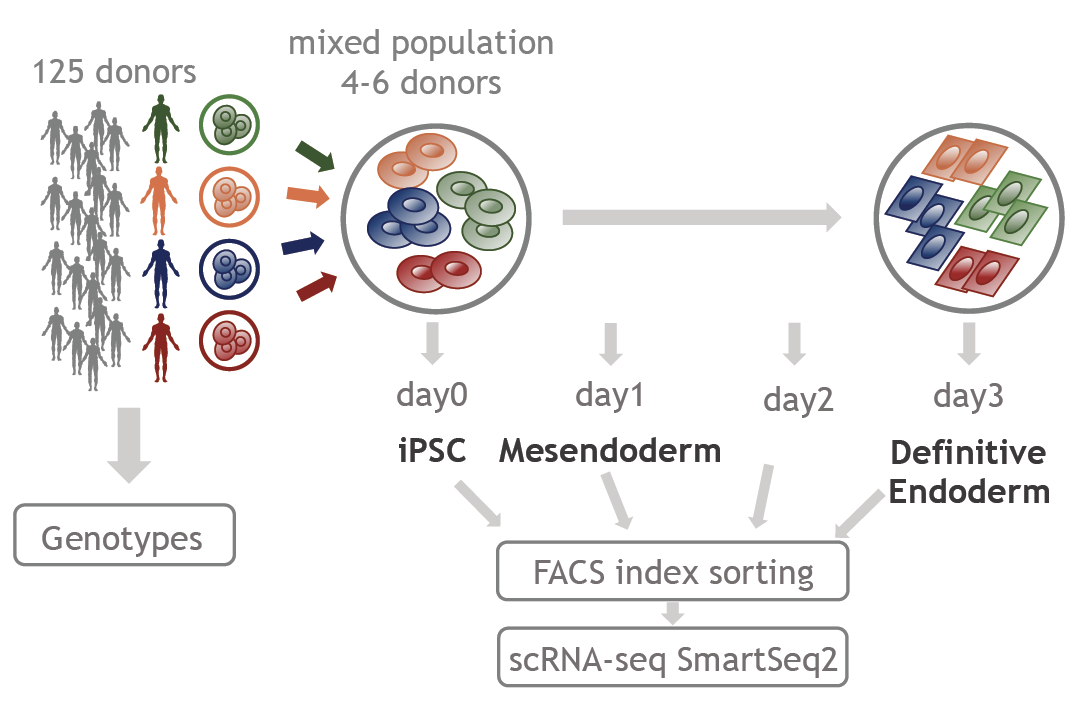
\includegraphics[width=12cm]{Chapter4/Fig/endodiff_experimental_design.png}
\caption[Experimental Design]{\textbf{Experimental Design}.\\
Human \gls{ipsc} lines from 125 unrelated donors were differentiated to definitive endoderm (\textbf{Fig. \ref{suppl_fig:endodiff_exp_protocol}}) using a pooled design, where cells from 4 to 6 lines were grown and differentiated together.
Cells were collected prior to differentiation (at day0) and every 24 hours along differentiation to definitive endoderm (at day1, day2 and day3).
Cells at day0 are expected to be pluripotent; cells at day1 are considered to be bipotent for either mesoderm or endoderm (mesendoderm); by day3, cells should have reached a definitive endoderm state.
At each time point, cells were FAC-sorted and sequenced using the SmartSeq2 technology.
\textcolor{blue}{Imputed genotypes} were also available for all lines.}
\label{fig:endodiff_experimental_design}
\end{figure}

% \subsection{Experimental strategy}

\subsection{Data processing and QC}
 
% add fast Q etc?

\subsubsection{Demultiplexing donors from pooled experiments} 

In the considered pooled experimental design, cells from multiple donors are differentiated together in the same experiment. 
To be able to link the genetic background of an individual with their transcriptional profile we need to map the cells back to their donor of origin, without the use of any barcode.
Indeed, we find that for the large majority of cells the RNA-seq reads map to a sufficient number of common genetic variants for us to reliably assign each cell to its original donor.
In particular, assignment of cells to donors was performed using Cardelino \cite{mccarthy2020cardelino}. 
In short, Cardelino estimates the posterior probability of a cell originating from a specific donor using common genetic variants in \gls{scrnaseq} reads, while employing a Bayesian beta binomial-based approach to account for technical factors such as differences in read depth, allelic drop-out, and sequencing accuracy. 
To perform donor assignment, we considered a larger set of \gls{hipsci} lines with genotype information (n=490), including the 126 lines used in this study. 
A cell's assignment to a donor was considered successful if the model identified the match i) with posterior probability > 0.9, and ii) using a minimum of 10 informative variants. 
Cells for which the donor identification was not successful were discarded and not considered for further analyses.
Across the entire dataset, 99\% of cells that passed RNA QC steps (see below) were successfully assigned to a donor.
In some cases, unexpected donor assignment (where several cells from one experiment were found to be assigned to none of the 4-6 donors used in that experiment) allowed me to identify (and correct) plate swaps that happened in the lab, without losing any data (\textbf{Fig. \ref{fig:plate_swap}}).

\begin{figure}[h]
\centering
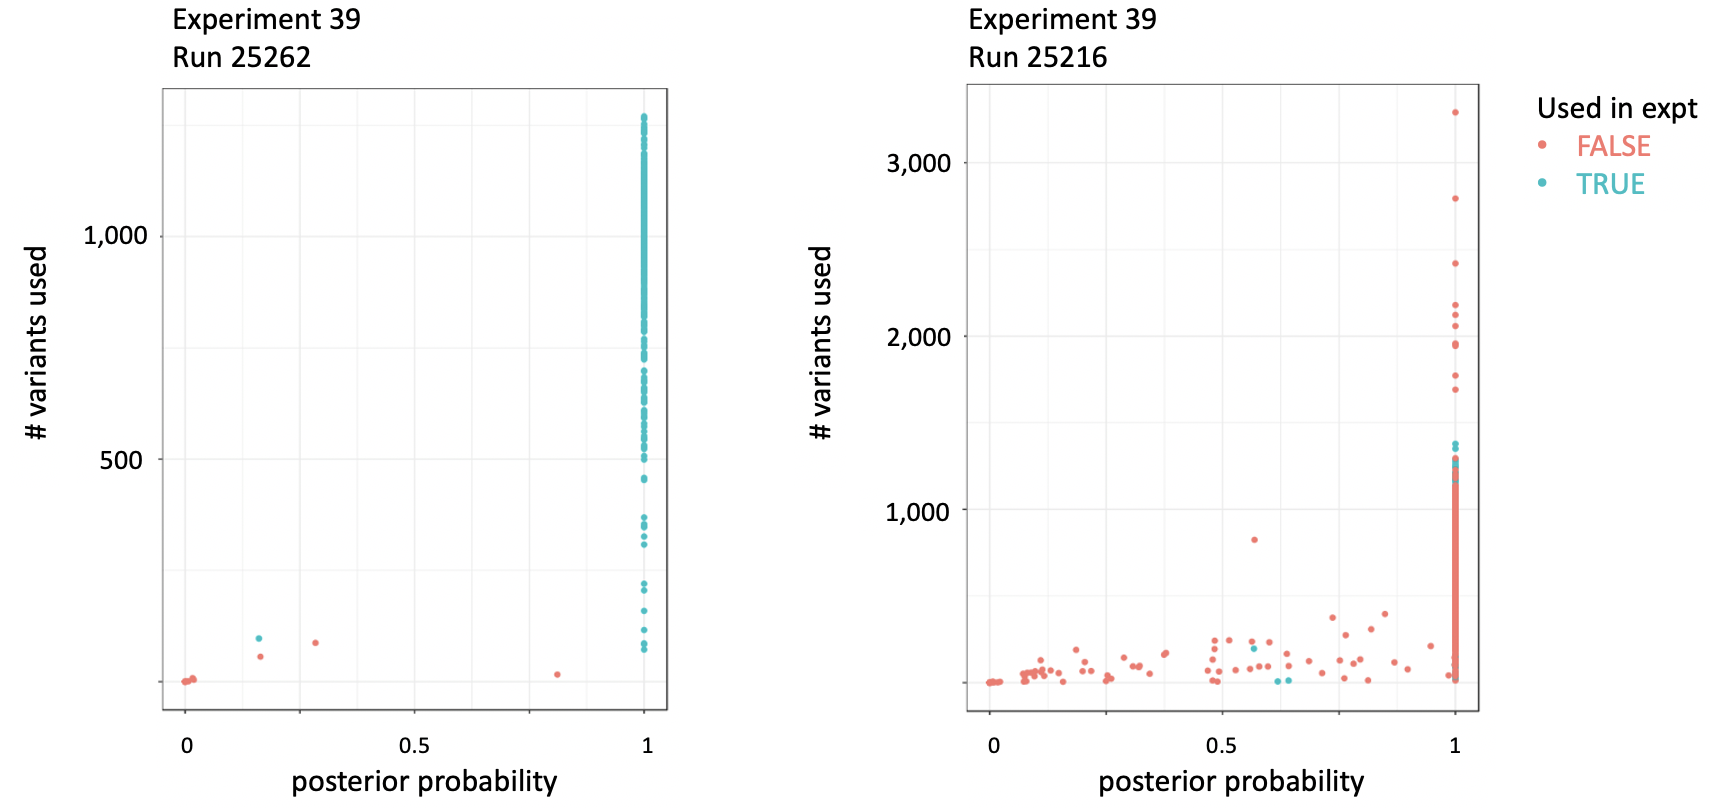
\includegraphics[width=14cm]{Chapter4/Fig/cardelino_example.png}
\caption[Demultiplexing donors]{\textbf{Demultiplexing donors}.\\
Example of how donor assignment of cells helped identifying a plate swap.
To explore the results of the donor assignment algorithm \cite{mccarthy2020cardelino}, I plotted cells along two axes: on the x axis, the posterior probability of being assigned to a certain donor, on the y the number of common variants found on \gls{scrnaseq} reads used to perform the assignment.
Because we know for each experiment which lines are supposed to have been differentiated, we can colour cells based on whether the donor they have been assigned to was used in the specific experiment or not.
On the left, an example of a correct donor assignment: most cells are assigned to one of the correct donors\footnotemark and the few that are not had very few usable genetic variants.
On the right, the donor assignment is apparently incorrect.
Most cells were assigned to donors that were not differentiated in the experiment, in many cases with a high level of confidence and using many variants, which would generally indicate high quality cells.
Indeed, investigating further we realised that all cells were assigned to donors that all belonged to the same experiment, but that it was a different experiment.
The wrong label was assigned in the lab: run 225216 actually contained cells from experiment 43 and not 39.
By resolving this computationally, we avoided mistakes and retained all of the cells from this sequencing run, which would have otherwise been discarded.}
\label{fig:plate_swap}
\end{figure}


\subsubsection{Flow cytometry}

The success of the differentiation protocol was validated using expression of two protein surface markers, a pluripotency marker, Tra-1-60, and a marker of definitive endoderm, CXCR4. 
We note that while cells were gated using the two markers, we did not discard any cells based on their expression. 
In contrast, the first cell QC step performed using \gls{facs} consisted in identifying dead cells based on 7AAD\footnote{Staining with 7AAD is used a cell viability assay.
7AAD cannot readily pass through intact cell membranes, thus only cells with compromised membranes will stain.} using \gls{facs} staining.
These were discarded and were not plated. 
\gls{facs} data were analysed using the openCyto package, implemented in R \cite{finak2014opencyto}.
The \gls{facs} gating strategy we used is illustrated in \textbf{Fig. \ref{fig:endodiff_facs_strategy}}.

\begin{figure}[h]
\centering
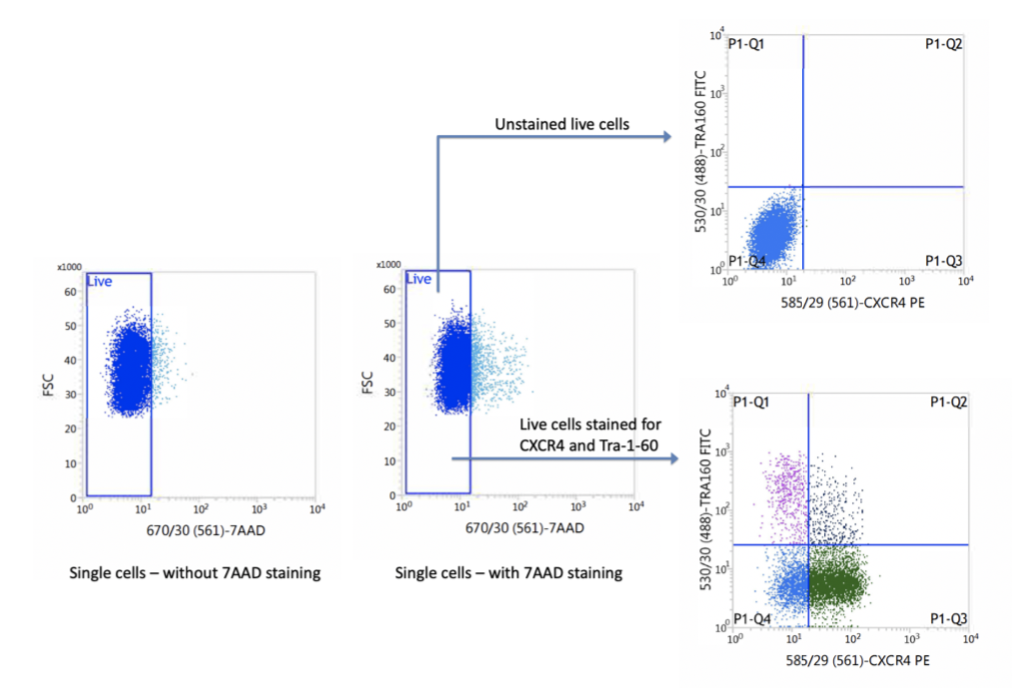
\includegraphics[width=14cm]{Chapter4/Fig/endodiff_facs_strategy.png}
\caption[FACS gating strategy]{\textbf{FACS gating strategy}.\\
Figure by Mariya Chhatriwala.
\gls{facs} gating strategy: first, single cells were stained with 7AAD to exclude dead cells. 
Unstained live cells were then used to gate for expression of Tra-1-60 and CXCR4.}
\label{fig:endodiff_facs_strategy}
\end{figure}

% Single cells/Doublets

\newpage

% footnote from plate swap figure (to make it appear on right page)
\footnotetext{A cell technically could still have been assigned to a wrong donor within the correct experiment, but given a threshold both on the variants used (> 10) and on the posterior probability (> 0.9) 
% we believe that this is 
I deemed this
unlikely.}

\subsubsection{scRNA-seq feature quantification and quality control}

Single cell profiles were obtained using the SmartSeq2 technology \cite{picelli2013smart}. 
This is a plate-based technology that involves single cells being sorted into 384 independent wells on a plate. 
Adaptors of raw \gls{scrnaseq} reads were trimmed using Trim Galore! \cite{galore2015wrapper, martin2011cutadapt, andrews2010fastqc}, using default settings. 
Trimmed reads were mapped to the human genome (build 37) using STAR \cite{dobin2013star}. 
Gene-level expression quantification was performed using Salmon \cite{patro2017salmon}. 
Briefly, Salmon quantifies transcript- (rather than gene-) level expression levels, similar to Kallisto \cite{bray2016near}.
Then, such values are summarised at a gene level (\gls{cpm}).\\

% \newpage

We performed \gls{qc} of \gls{scrnaseq} profiles following a widely used pipeline (see \textbf{section \ref{sec:scrnaseq}}) using Bioconductor packages \textit{scater} and \textit{scran}, implemented in R \cite{lun2016step, mccarthy2017scater, lun2019singlecellexperiment}.  
In particular, cells were retained for downstream analysis if they had at least 50,000 counts from endogenous genes, at least 5,000 genes with non-zero expression, if less than 90\% of counts came from the top 100 most highly-expressed genes, less than 15\% of reads mapped to mitochondrial (MT) genes, they had a Salmon mapping rate of at least 60\%, based on distribution observation and thresholding (\textbf{Fig. \ref{fig:endodiff_qc_distributions}}) \cite{luecken2019current}.
Additionally, cells were only retained if they could be successfully assigned to a donor (QC1, \textbf{Fig. \ref{fig:endodiff_qc_workflow}}). \\ 

I then performed an additional QC step, where I excluded all cells from plates and experiments that had overall low quality.
In the case of plates sequenced twice, I retained the one with most cells.
Finally, I retained plates that had enough cells for the majority of the donors considered (QC2, \textbf{Fig. \ref{fig:endodiff_qc_workflow}}). 

\begin{figure}[h]
\centering
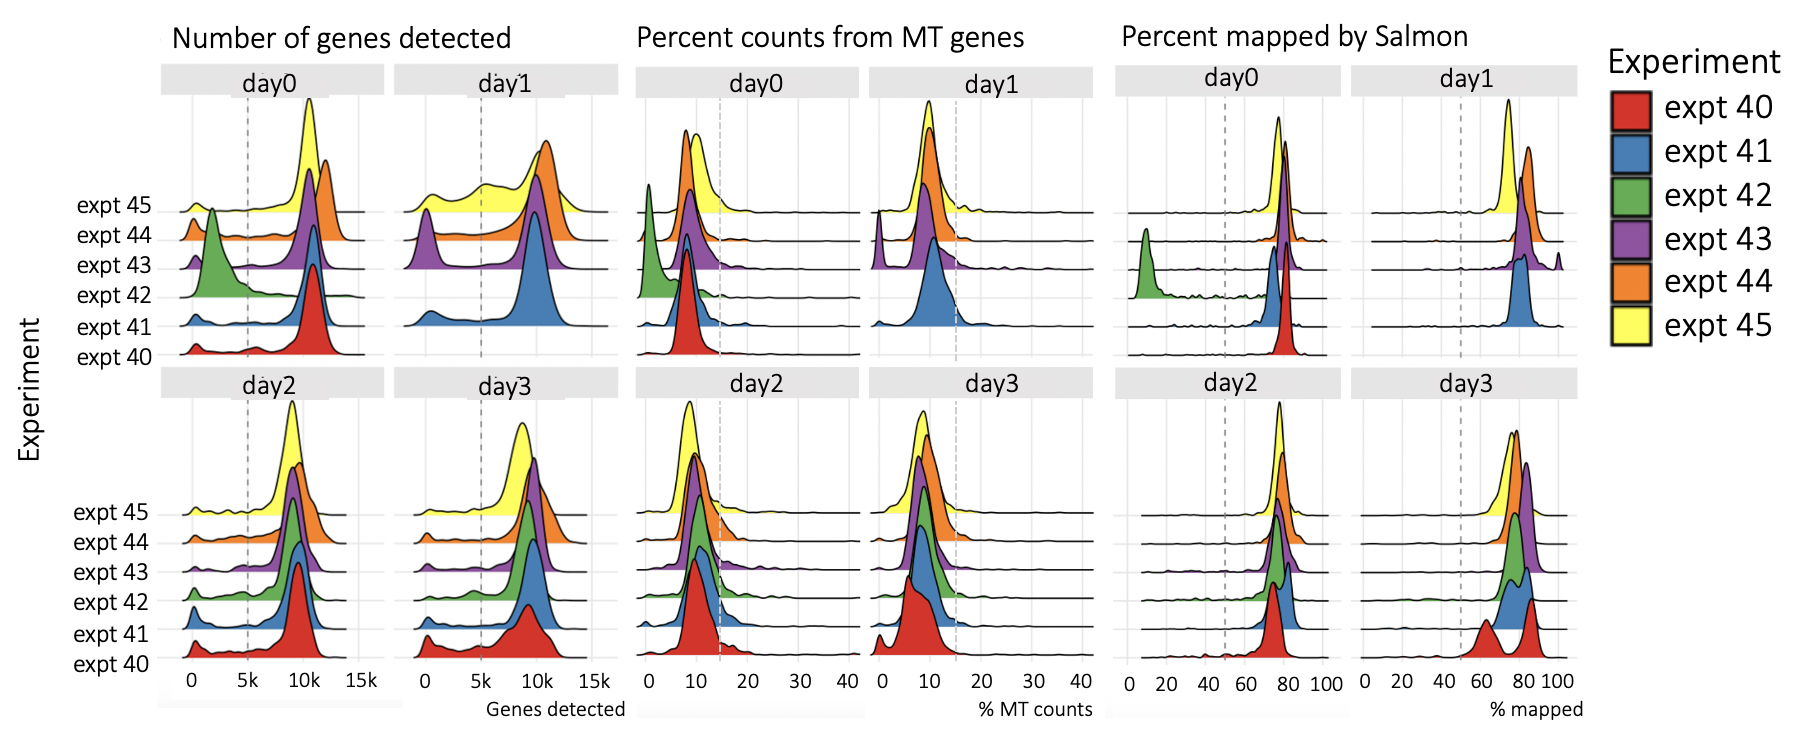
\includegraphics[width=16cm]{Chapter4/Fig/endodiff_qc_examples.png}
\caption[Distributions of QC metrics]{\textbf{Distributions of QC metrics}.\\
Distributions of three exemplar QC metrics for six differentiation experiments (40-45).
Shown are the cell distributions along the metrics (number of genes detected, percentage of counts from mitochondrial genes, Salmon \cite{patro2017salmon} mapping rate), as well as the thresholds we used as dotted lines, stratified by day and experiment.
One can immediately spot how poor quality plates\footnotemark  perform similarly badly across all metrics (i.e. < 5,000 genes detected, <60\% reads mapped by Salmon).}
\label{fig:endodiff_qc_distributions}
\end{figure}

\begin{figure}[h]
\centering
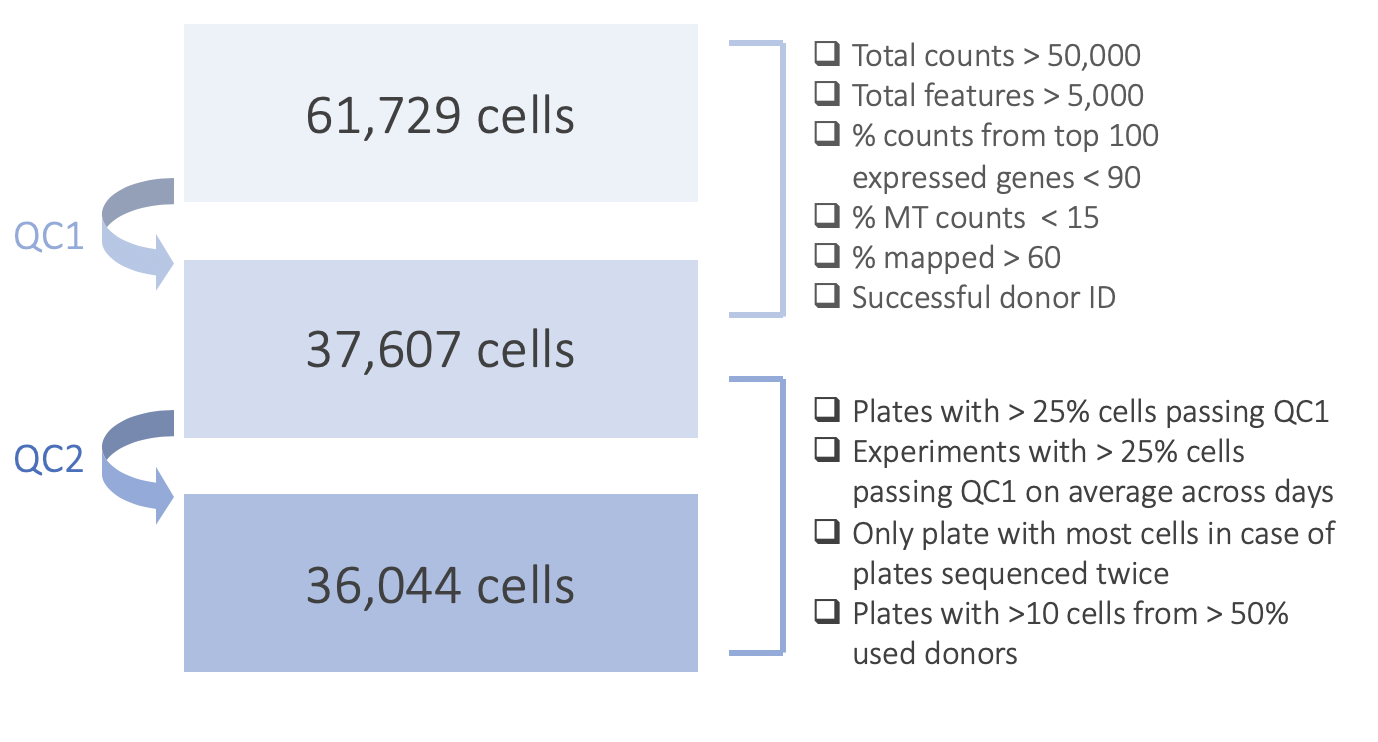
\includegraphics[width=16cm]{Chapter4/Fig/endodiff_qc_workflow.png}
\caption[QC workflow]{\textbf{QC workflow}.\\
Two stages of cell QC.
First, at the level of single cells, all QC metrics and thresholds are indicated.
61\% of cells passed QC1.
Second, at the experiment/plate level.
If plates had many cells not passing QC1 they were considered poor quality batches and removed altogether.
This stage removed far fewer cells, with 96\% of cells considered passing QC2.}
\label{fig:endodiff_qc_workflow}
\end{figure}

\subsubsection{scRNA-seq processing}

SmartSeq2 data do not include \glspl{umi}, which can be used to accurately detect PCR duplicates and quantify transcript abundance \cite{smith2017umi, islam2014quantitative, kivioja2012counting}. 
In the absence of \glspl{umi}, we can borrow information from cells with similar total number of reads and correct for overall library size. 
Such size factor normalisation of counts was performed using \textit{scater} \cite{mccarthy2017scater}.
% \cite{lun2016pooling}?
\\

Expressed genes with an HGNC symbol were retained for analysis, where expressed genes in each batch of samples were defined based on (i) raw count >100 in at least one cell prior to cell QC (i.e. \textbf{Fig. \ref{fig:endodiff_qc_workflow}}) and (ii) average log2(CPM+1) >1 after cell QC. 
Normalised CPM data were log transformed (log2(CPM+1)) for all downstream analyses. 
% The joint dataset was investigated for outlier cell lines/donors or experiments, identifying no clear groups of outlying cells. 
As a last QC step, we considered possible differences between cell lines derived from healthy and diseased donors. 
Specifically, a subset of 11 cell lines in our dataset were derived from monogenic neonatal diabetes patients, and differentiated together with cell lines from healthy donors across 7 differentiation experiments (out of 28). 
There was no significant difference in differentiation efficiency (see \textbf{section \ref{sec:endodiff_differentiation_efficiency}}) between healthy and neonatal diabetes lines in these experiments (p value > 0.05), and cells from both sets of donors overlapped in principal component space (\textbf{Fig. \ref{suppl_fig:pca_diabetes_lines}}). 
Thus, we included cells from all donors in our analyses, irrespective of disease state.
% The final merged and QC’ed dataset consisted of 36,044 cells with expression profiles for 11,231 genes.


% \section{Results}
\newpage

\section{Data overview}
\label{sec:endodiff_overview}

%  We considered a panel of well-characterised human \gls{ipsc} lines derived from 125 unrelated donors from the \gls{hipsci} collection \cite{kilpinen2017common}. 
%  In order to increase throughput and mitigate the effects of batch variation, we exploited a novel pooled differentiation assay, combining sets of four to six lines in one well prior to differentiation (28 differentiation experiments performed in total; hereon “experiments”; Fig. 1A). 
%  Cells were collected at four differentiation time points (iPSC; one, two and three days post initiation - hereon day0, day1, day2 and day3) and their transcriptomes were assayed using full-length RNA-sequencing (Smart-Seq2 \cite{picelli2013smart}) alongside the expression of selected cell surface markers using \gls{facs} (TRA-1-60, CXCR4). 
Following quality control (QC), 36,044 cells were retained for downstream analysis, across which 11,231 genes were expressed.
%  Exploiting the observation that each cell line’s genotype acts as a unique barcode, we demultiplexed the pooled cell populations, enabling identification of the cell line of origin for each cell (similar to \cite{kang2018multiplexed}). 
At each time point, cells from between 104 and 112 donors were captured, with each donor being represented by an average of 286 cells (after QC, \textbf{Fig. \ref{fig:endodiff_stats}}). 
The success of the differentiation protocol was validated using canonical cell-surface marker expression: consistent with previous studies \cite{chu2016single}, an average of 72\% of cells were TRA-1-60(+) in the undifferentiated state (day0) and an average of 49\% of cells were CXCR4(+) three days post differentiation (day3, \textbf{Fig. \ref{fig:endodiff_stats}}).
 
\begin{figure}[htbp]
\centering
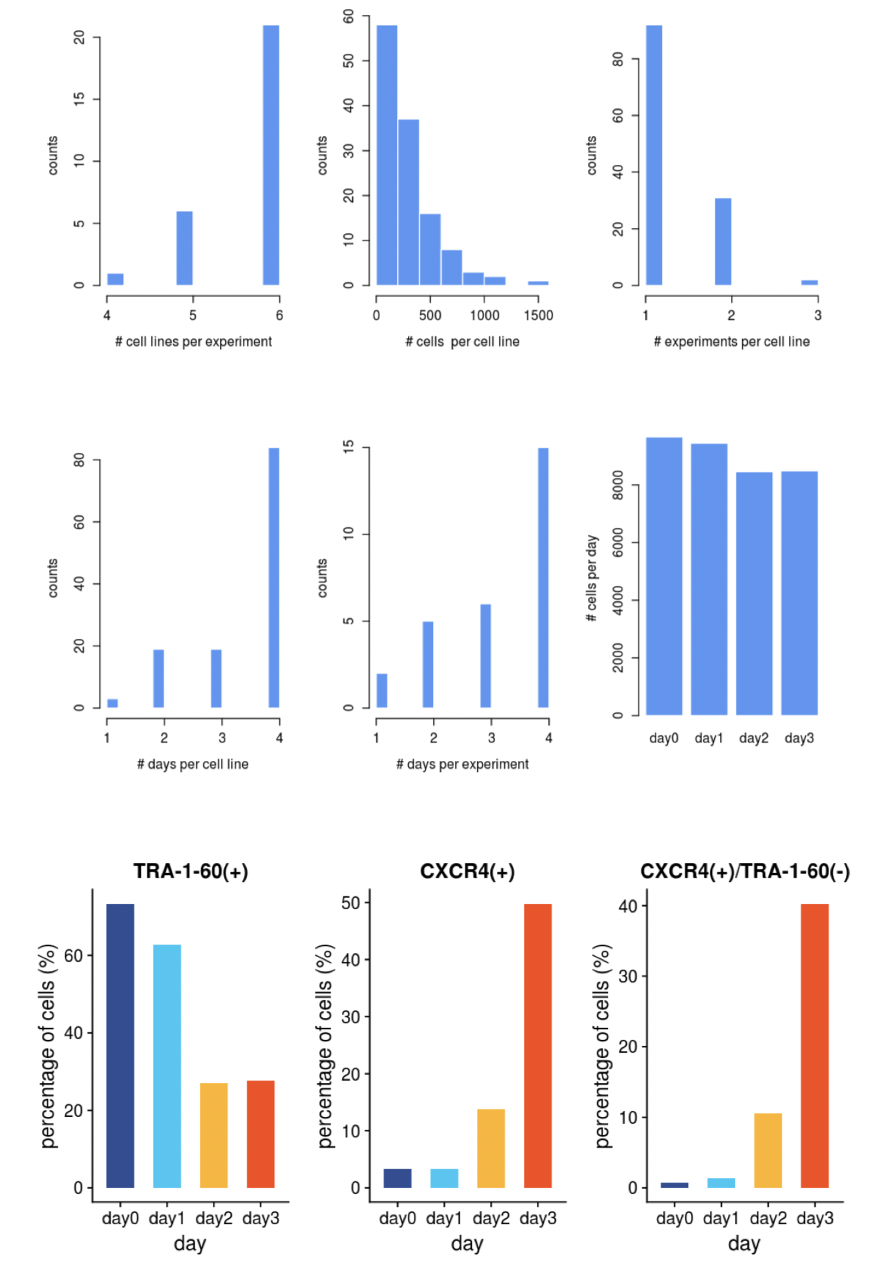
\includegraphics[width=14cm]{Chapter4/Fig/endodiff_stats.png}
\caption[Overview of experimental metrics]{\textbf{Overview of experimental metrics.}\\
Statistics for number of cells, donors, experiments, days, and combinations. 
Cell counts are shown after quality control.
Additionally, shown are the percentages of cells that are positive for TRA-1-60, a pluripotency marker, positive for CXCR4, a definitive endoderm marker, and  positive for CXCR4 and negative for TRA-1-60, across all cell lines and all experiments.}
\label{fig:endodiff_stats}
\end{figure}

 % footnote from qc examples figure (to make it appear on right page)
\footnotetext{e.g. cells from day0, experiment 42. }

\newpage

\subsection{Sources of variation} 
\label{sec:endodiff_sources_of_variation}

% \begin{wrapfigure}{r}{0.6\textwidth}
% 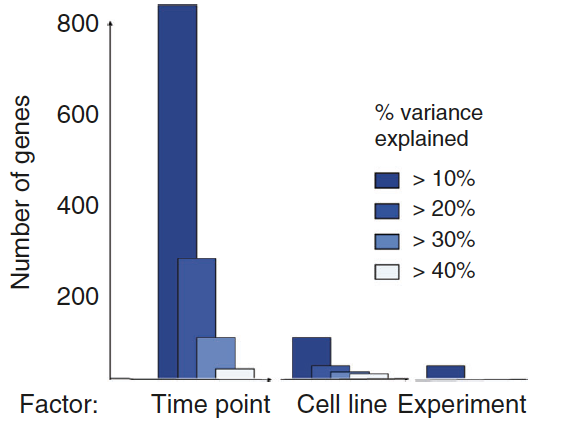
\includegraphics[width=9cm]{Chapter4/Fig/endodiff_variance_component.png}
% \caption[Variance Component Analysis]{\textbf{Variance Component Analysis}.\\
% Variance component analysis of 4,546 highly variable genes, using a linear mixed model fit to individual genes to decompose expression variation into
% time point of collection, cell line and experimental batch.}
% \label{fig:endodiff_vca}
% \end{wrapfigure}

To identify the main sources of variation in our dataset we performed variance component analysis for each of the genes, using a linear mixed model.
Variance component analysis revealed the time point of collection as the main source of variation, followed by the cell line of origin and the experimental batch (\textbf{Fig. \ref{fig:endodiff_vca}}).\\

\begin{figure}[h]
% \centering
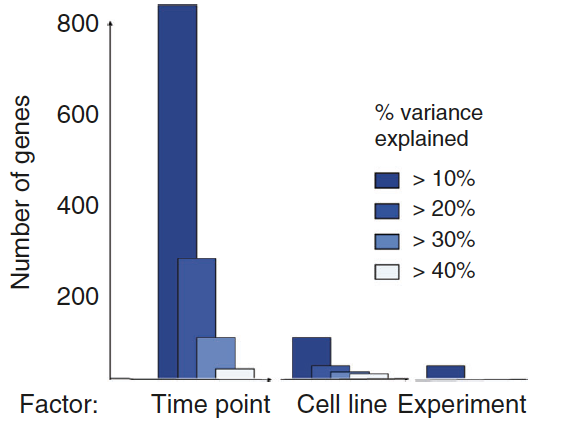
\includegraphics[width=10cm]{Chapter4/Fig/endodiff_variance_component.png}
\caption[Variance Component Analysis]{\textbf{Variance Component Analysis}.\\
Summary of variance component analysis results for each of 4,546 highly variable genes, using a linear mixed model fit to individual genes to decompose expression variation into
time point of collection, cell line and experimental batch.
The number of genes for which each factor explains 10\%, 20\%, 30\% and 40\% of the variance respectively is indicated.}
\label{fig:endodiff_vca}
\end{figure}

Next, we performed \gls{pca} on our dataset.
To do so, we first identified the top 500 \gls{hvgs} defined as the most variable genes given a mean-variance trend calculated across all genes, using the function \textit{trendVar} as implemented in the R package scran.
Consistent with the results from the variance component analysis (\textbf{Fig. \ref{fig:endodiff_vca}}), the first principal component (PC1) was aligned with differentiation time, motivating its use to order cells by their differentiation status (hereafter `pseudotime', \textbf{Fig. \ref{fig:endodiff_pca}}).\\

\begin{figure}[h]
\centering
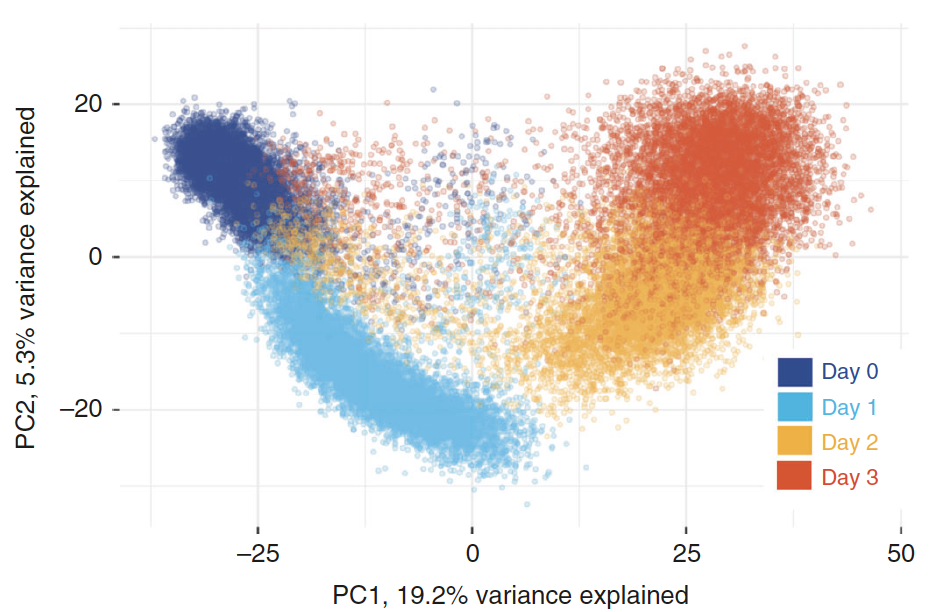
\includegraphics[width=14cm]{Chapter4/Fig/endodiff_pca_overview.png}
\caption[Overview of dataset.]{\textbf{Overview of dataset.}\\
Principal component analysis of gene expression profiles for 36,044 QC-passing
cells, coloured by the time point of collection.
PC1 effectively captures differentiation time and is defined as pseudotime.}
\label{fig:endodiff_pca}
\end{figure}

Pseudotime inference is a common step in the analysis of \gls{scrnaseq} data along differentiation and development: while single cells are single snapshots along time, with enough points and considering that cells differentiate at different rates, they can be used to reconstruct a trajectory.
In this case, the nature of the short and linear differentiation process of our data (i.e. iPSC $\rightarrow$ mesendoderm $\rightarrow$ definitive endoderm) meant that PC1 captured the differentiation trajectory.
For comparison, we did apply alternative pseudotime inference methods, which yielded similar orderings (\textbf{Fig. \ref{fig:endodiff_pseudotimes}}).
Further validation of our inferred pseudotime was provided by the temporal expression dynamics of known marker genes that characterise endoderm differentiation, which was captured by our ordering of cells as expected (\textbf{Fig. \ref{fig:endodiff_stages}}).

\begin{figure}[htbp]
\centering
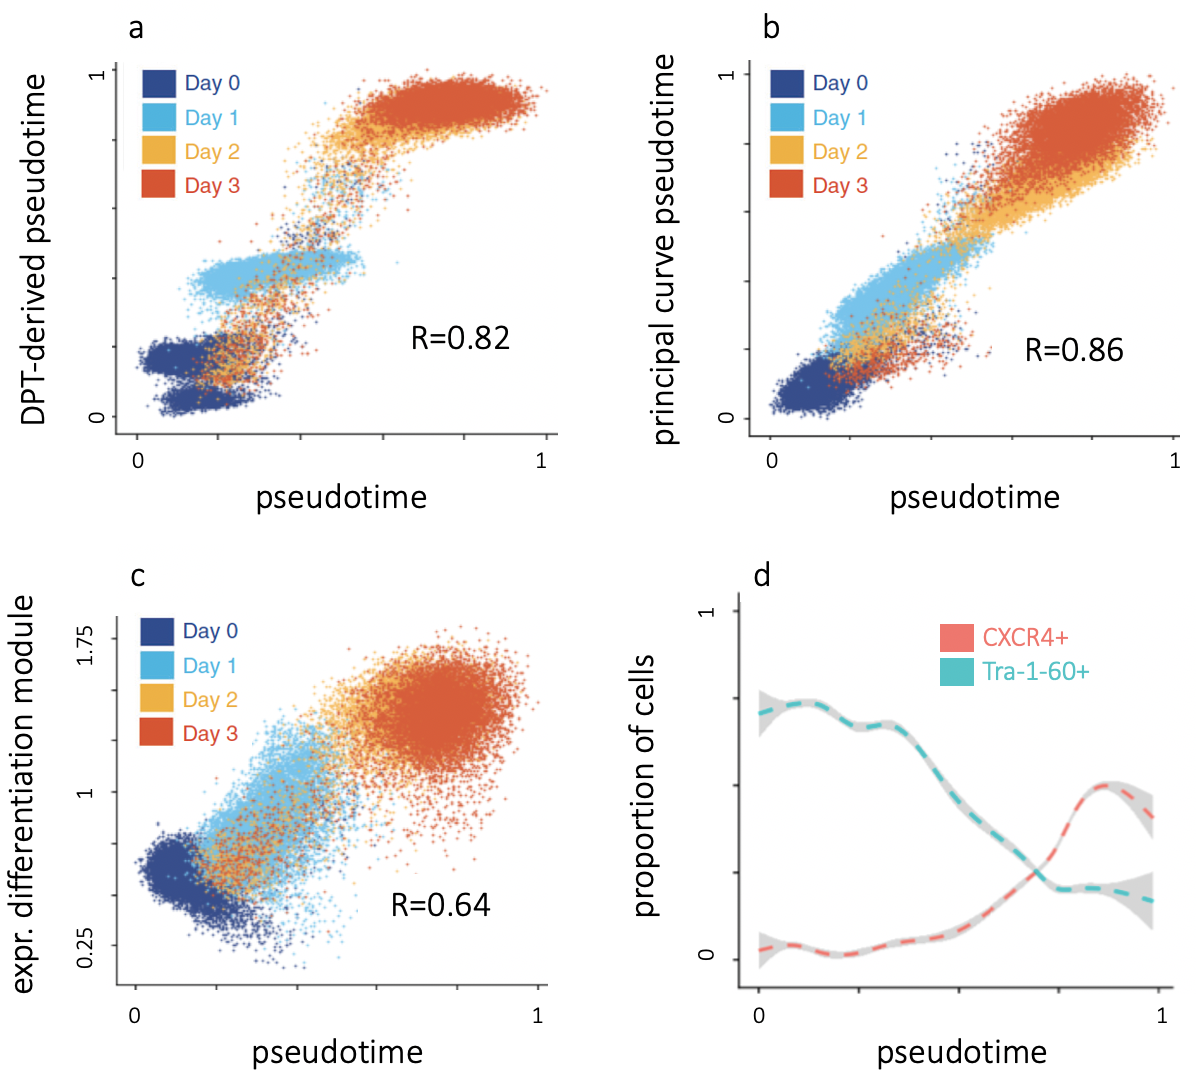
\includegraphics[width=14cm]{Chapter4/Fig/endodiff_pseudotimes.png}
\caption[Evaluation of pseudotime definition]{\textbf{Evaluation of pseudotime definition by comparison with alternative approaches.}\\
(a) Comparison of the pseudotime defined based on principal component analysis with diffusion pseudotime (DPT) \cite{haghverdi2016diffusion}. 
The diffusion map was generated using 15 nearest neighbours and the first 20 PCs across the top 500 most highly variable genes.  
(b) Comparison of our defined pseudotime with an alternative measure of pseudotime based on projection of each cell on to a principal curve (using princurve as implemented in R \cite{hastie1989principal}) calculated using the first two principal components from the top 500 most highly variable genes. 
(c) Comparison of our pseudotime to the average expression of 124 co-expressed genes associated with cell differentiation. 
(d) Scatter plot-derived loess curves of \gls{facs} markers as a function of the our PCA-based pseudotime, showing expected trends.}
\label{fig:endodiff_pseudotimes}
\end{figure}

\subsection{Defining discrete developmental stages}

While the continuous measure of pseudotime nicely highlights the dynamics of gene expression over time, in order to map eQTL, and to be able to exploit methods similar to those described in the previous chapter (\textbf{Chapter 
\ref{chapter3}}),
% 3), 
it was also important to define homogeneous populations of cells that represent specific developmental stages.
To do so, we assign our cells to one of three non-overlapping stages, corresponding to the three canonical stages of endoderm differentiation: \gls{ipsc}, mesendoderm (mesendo) and definitive endoderm (defendo).
In particular, we utilise i) the ordering of cells along our inferred pseudotime ii) the expression of the previously described markers of differentiation progress and iii) the cell's day of collection to determine the cell assignment to each stage (\textbf{Fig. \ref{fig:endodiff_stages}}).

Specifically, we assign all day0 cells to the iPSC cluster given their very high homogeneity.
Next, cells were assigned to the mesendoderm stage if they were collected at either day1 or day2, and had pseudotime values corresponding to the peak expression of \textit{Brachyury} (\textit{T}) along pseudotime (pseudotime between 0.15 and 0.5, \textbf{Fig. \ref{fig:endodiff_stages}}).  
Similarly, cells were assigned to definitive endoderm if they were collected at day2 or day3 and had pseudotime values higher than 0.7, corresponding to a pseudotime window with maximal expression of \textit{GATA6} (\textbf{Fig. \ref{fig:endodiff_stages}}).
In total, we assigned 28,971 cells (about $\sim$80\% of all cells) to one of the three stages. 
A smaller fraction of cells with intermediate pseudotime (between 0.5 and 0.7, n=7,073) could not be confidently assigned to a canonical stage of differentiation; these cells were largely collected at day2, at which stage rapid changes in expression profiles are expected, reflecting a transitional population of cells.
We note that these cells were excluded for the purposes of the initial stage eQTL mapping (results in \textbf{section \ref{sec:endodiff_eqtl}}), but are included in all other analyses. 

\vspace{2mm}

\begin{figure}[h]
\centering
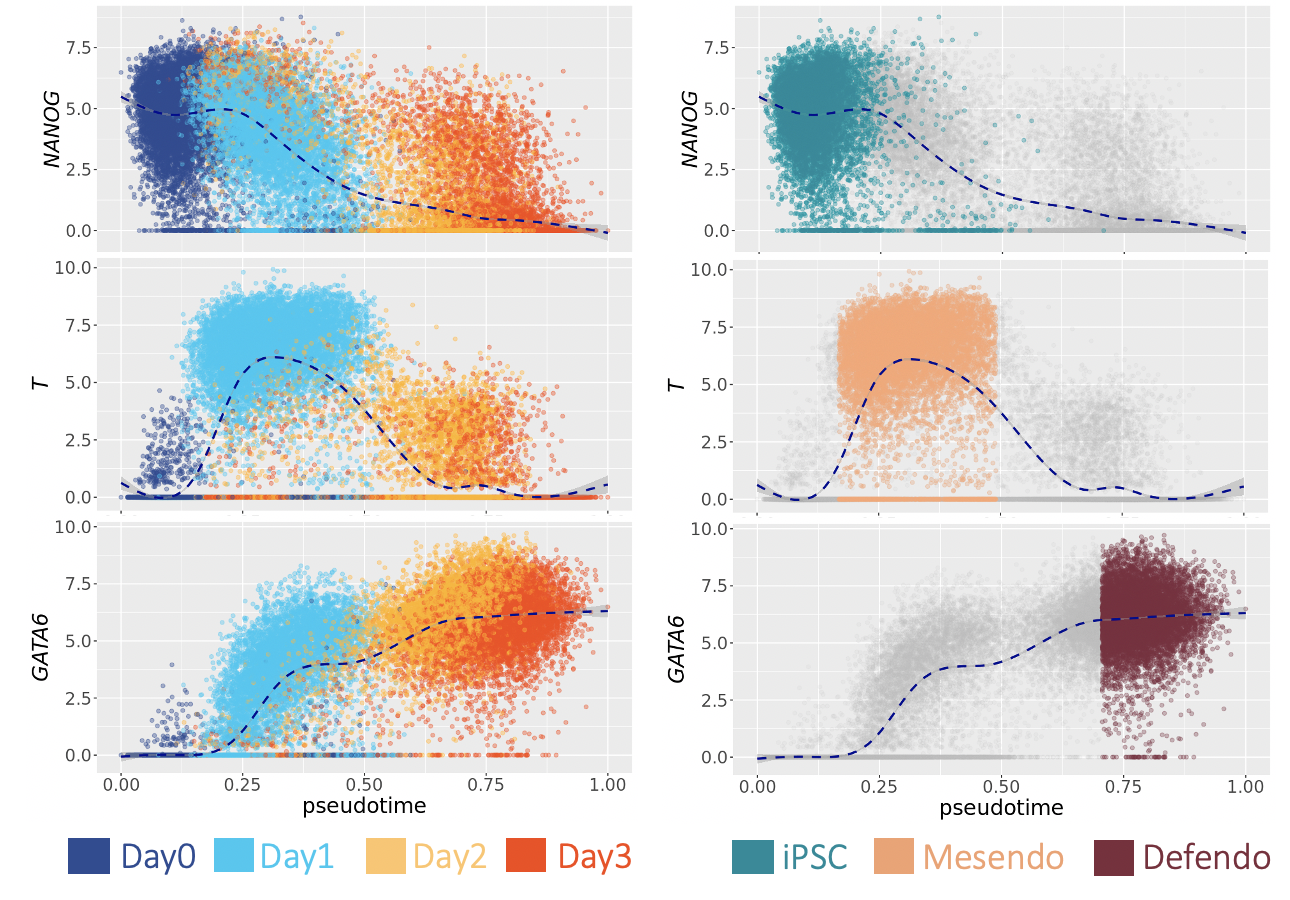
\includegraphics[width=14cm]{Chapter4/Fig/endodiff_stages.png}
\caption[Developmental stages]{\textbf{Marker gene expression in pseudotime-based developmental states.}\\
Expression of exemplar canonical markers for iPSC (\textit{NANOG}), mesendoderm (\textit{T}) and definitive endoderm (\textit{GATA6}) along pseudotime.
Developmental stages were defined taking into consideration i) the day of collection, ii) the expression of canonical markers, and iii) the position along pseudotime.}
\label{fig:endodiff_stages}
\end{figure}

\section{Mapping eQTL in iPSCs, mesendo and defendo}
\label{sec:endodiff_eqtl}

By combining single cell expreesion profiling and common genetic variation of over one hundred individuals we can begin to assess the impact of genetic variability on expression in a continuous manner across early human development.
We have imputed genotypes for all of our 125 samples \cite{kilpinen2017common}, so this study allows discovery of single cell eQTL along differentiation. 
% This was partly motivated by the observation that a substantial fraction of variability in gene expression was explained by cell-line effects (\textbf{Fig. \ref{fig:endodiff_vca}}).
% \subsection{Mapping eQTL}
Using the developmental stages just described and methods similar to those described in the previous chapter, we mapped eQTL in each of the \gls{ipsc}, mesendo and defendo populations, yielding 1,833, 1,702 and 1,342 eGenes, respectively. 
Briefly, we quantified each gene’s average expression level for each donor, experiment, and differentiation stage\footnote{This approach is the same as what is described in the first part of \textbf{Chapter \ref{chapter3}}, and similar to the `mean' described in \textbf{section \ref{sec:best_practice}}, except that the aggregation is done at the experiment level rather than the sequencing run level.}, before using a linear mixed model to test for \textit{cis} eQTL, adapting approaches used for bulk RNA-seq profiles (+ and - 250 kb, MAF >5\% \cite{kilpinen2017common}).\\

For comparison, we also performed eQTL mapping in cells collected on day1 and day3, i.e. the experimental time points commonly used to identify cells at mesendo and defendo stages \cite{hannan2013production}.
% mention that this can be partially explained by differences in differentiation rate for different individuals etc?
Interestingly, this approach identified markedly fewer eGenes: 1,181 eGenes at day1, and 631 eGenes at day3.
These results demonstrate the power of using the single-cell RNA-seq profiles to define relatively homogeneous differentiation stages in a data-driven manner (\textbf{Fig. \ref{fig:endodiff_stage_eqtl}}). 
Notably, this observation was not merely a consequence of differences in the number of cells or donors considered in each cell population (\textbf{Fig. \ref{fig:endodiff_stage_eqtl}}). \\

\begin{figure}[h]
\centering
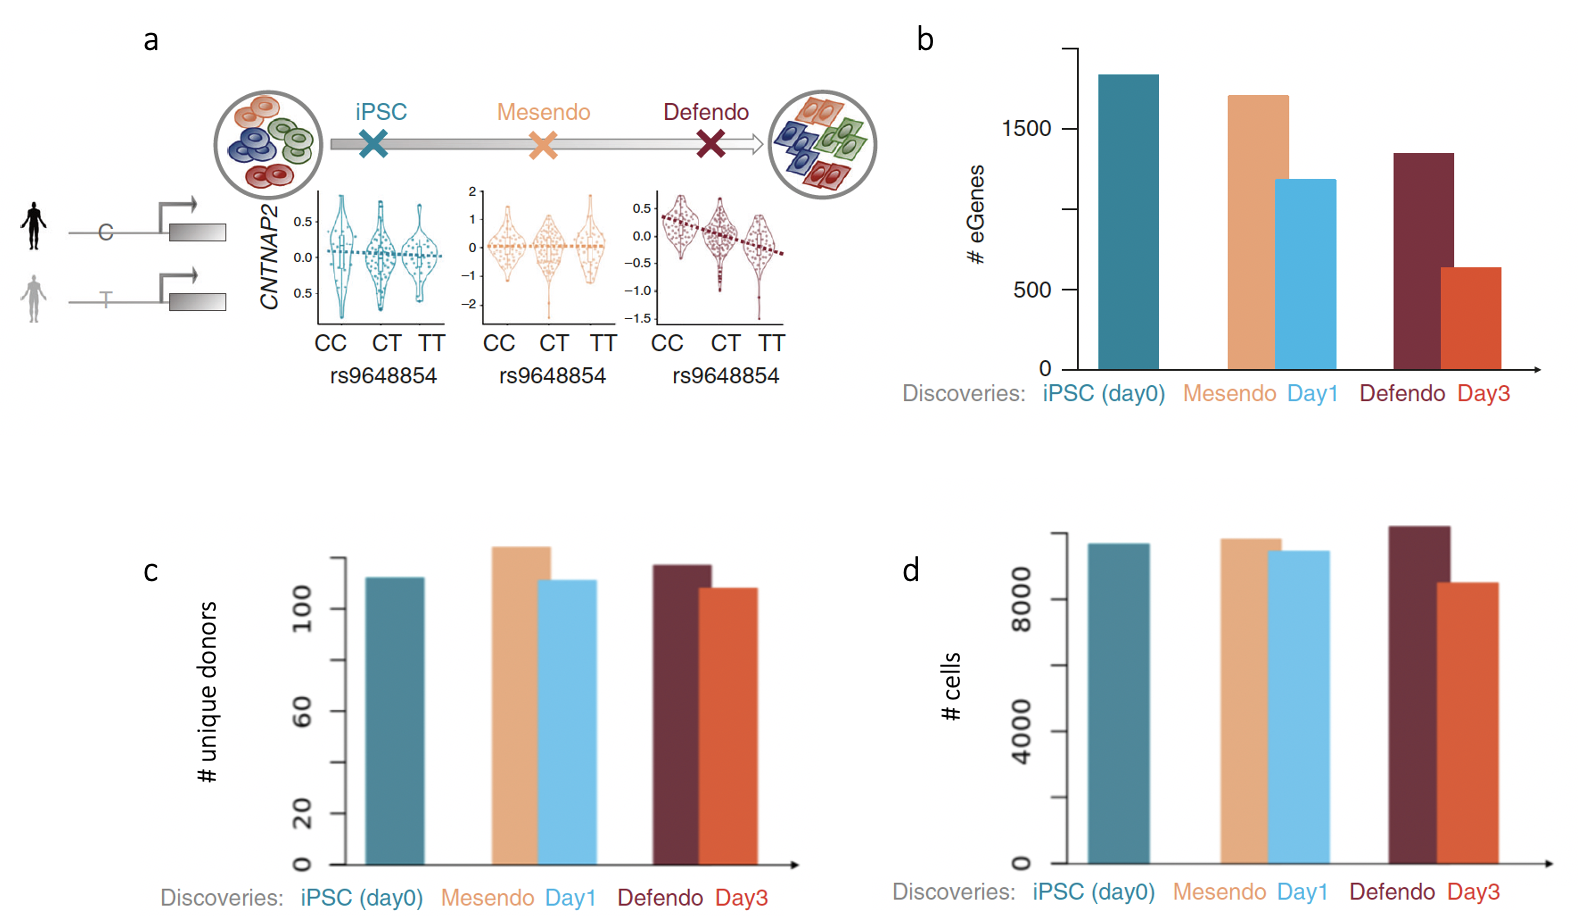
\includegraphics[width=14cm]{Chapter4/Fig/endodiff_eqtl.png}
\caption[eQTL maps of iPSC, mesendo, defendo]{\textbf{Mapping single cell eQTL at different developmental stages.}\\
(a) Illustration of the single cell eQTL mapping strategy at various stages of differentiation.
Shown is an example of a defendo-specific eQTL. 
Box plots of gene expression stratified by the allelic state of
rs9648854 at each stage, showing an association between rs9648854 and \textit{CNTNAP2} expression at the defendo stage, but not at earlier stages. 
(b) Comparison of eQTL mapping using different strata of all cells.
The use of pseudotime-based stages increases the number of detectable eQTL, compared to using the corresponding time point of collection.
Bar plots represent number of eGenes (genes with at least one eQTL, at FDR < 10\%).
(c) Similar to b, the number of donors for which gene expression data were assayed at day0, day1, and day3, compared to the number of donors in the pseudotime-inferred mesendo and defendo stages.
(d) As for (c), with the number of cells.
\url{https://github.com/ebiwd/EBI-Icon-fonts} by EBI Web Development is licensed under CC BY 4.0. }
\label{fig:endodiff_stage_eqtl}
\end{figure}

% rephrase all of the below
% bulk it up so that it takes the whole last page
Profiling multiple stages of endoderm differentiation allowed us to assess at which stage along this process individual eQTL can be detected as well as the level of sharing of genetic signal across time. 
We observed substantial regulatory and transcriptional remodelling upon endoderm differentiation of iPSCs, with over 30\% of eQTL being specific to a single stage.
To define pairwise replication (and conversely specificity) between two sets of test results we considered nominal significance (p value < 0.05) and consistent direction of the effect size.
Importantly, we observed that stage-specificity of eQTL was not significantly explained by stage-specific gene expression (\textbf{Fig. \ref{fig:endodiff_stage_specific_eqtl}}).
Our differentiation time course covers developmental stages that have never before been accessible to genetic analyses of molecular traits and thus this study provides the first eQTL maps at mesendoderm and definitive endoderm.
We next explored whether any of the eQTL identified in these two studies were novel, and found that 349 of them have not been reported in either a recent iPSC eQTL study based on bulk RNA-seq \cite{mirauta2018population}, or in a compendium of eQTL identified from 49 tissues as part of the GTEx project \cite{gtex2017genetic}.
An eQTL was defined as novel when it was not reported as lead variant (FDR < 10\%) in any of the tissues considered nor was it in \gls{ld} (see \textbf{section \ref{sec:gwas}}) with any reported lead variant, \gls{ld} assessed using $r^2<0.2$.\\

Finally, we investigated the presence of lead switching events.
These correspond to two distinct genetic variants that are identified as lead eQTL for the same gene at different stages of differentiation (at LD: $r^2<0.2$),
We found lead switching events for 155 eGenes (an example in iPSC and defendo is illustrated in \textbf{Fig. \ref{fig:endodiff_stage_specific_eqtl}}). 
To explore the potential regulatory role of these variants, we investigated whether the corresponding genetic loci also featured changes in histone modifications during differentiation. 
To do so, we used ChIP-Sequencing to profile five histone modifications that are associated with promoter and enhancer usage (H3K27ac, H3K4me1, H3K4me3, H3K27me3, and H3K36me3) \textcolor{blue}{in human embryonic stem cells (hESCs)} that were differentiated towards endoderm (using the same protocol employed above) and measured at equivalent time points (i.e. day0, day1, day2, day3, \textcolor{blue}{see \textbf{section \ref{sec:endodiff_chipseq}} for detailed experimental methods)}. 
Interestingly, we observed corresponding changes in the epigenetic landscape for 20 of the lead switching events (i.e. stage-specific lead variants overlapped with stage-specific changes in histone modification status), suggesting a direct mechanism (\textbf{Fig. \ref{fig:endodiff_stage_specific_eqtl}}).

\begin{figure}[htbp]
\centering
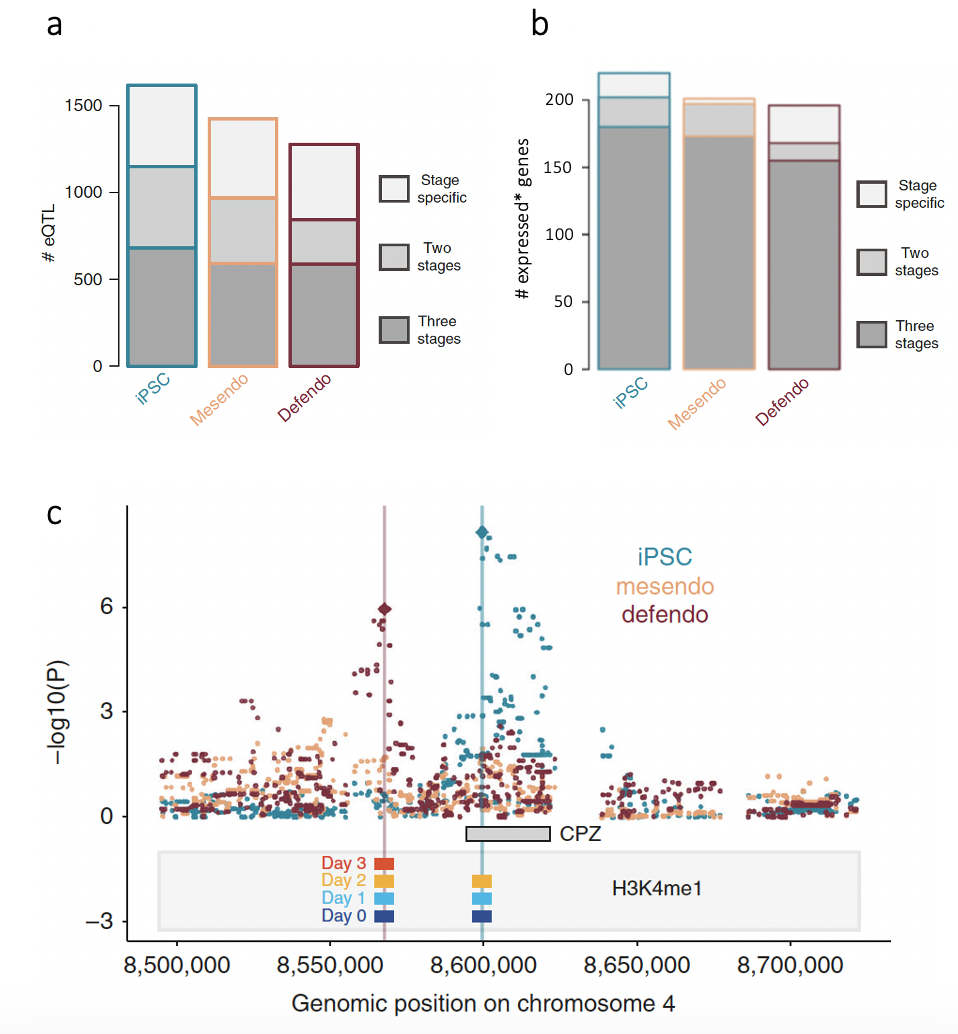
\includegraphics[width=12cm]{Chapter4/Fig/endodiff_stage_specific.png}
\caption[Stage-specific eQTL]{\textbf{Stage-specific eQTL.}\\
(a) Proportion of eQTL that are specific to a single stage, shared across two
stages, or observed across all stages (sharing defined as a lead eQTL variant at one stage with nominal p value < 0.05 and consistent direction
at another stage).
(b) Proportion of stage-specific eGenes (genes with a stage-specific eQTL) that are expressed only at a single stage, expressed at two stages, or expressed at all stages. 
Expressed is defined as normalised log2(CPM+1) > 2. 
CPM: counts per million.
(c) A lead switching event consistent with epigenetic remodelling. 
The overlap of H3K4me1 with the eQTL SNPs across differentiation time points is shown by the coloured bars.}
\label{fig:endodiff_stage_specific_eqtl}
\end{figure}

\newpage

\section{Dynamic eQTL across iPSC differentiation}
\label{sec:endodiff_dynamic_eqtl}

The availability of large numbers of cells per donor across a continuous differentiation trajectory from pluripotent stage to definitive endoderm enabled the analysis of dynamic changes of eQTL strength at fine-grained resolution. 
% \\
% add brief paragraph on ASE to quantify genetic effects and refer to box
% (fill the page) rearranged so borrow bits from below (sliding window)
To formally test for eQTL effects that change dynamically across differentiation (dynamic eQTL), we tested for associations between pseudotime (both linear and quadratic) and the genetic effect size using allele-specific expression (ASE) and a linear model (see \textbf{Box \ref{box:ase}}):
% In parallel, we reassessed each eQTL in each window taking advantage of the full length transcript sequencing to measure allele-specific expression (ASE).

\begin{equation}\label{eq:endodiff_ase_pseudotime}
    \mathrm{ASE} = \alpha_1 \mathrm{pseudotime} + \alpha_2 \mathrm{pseudotime}^2 + \boldsymbol{\psi},
\end{equation}

\textcolor{blue}{where the genetic effect is defined based on \gls{ase} at the level of single cells, i.e. quantified as fractional read counts overlapping each allele for a given gene-SNP pair (see details in \textbf{Box \ref{box:ase}}).}
We assessed significance using a likelihood ratio test with two degrees of freedoom (i.e. $H_0: \alpha_1 = \alpha_2 = 0$). 
For this analysis, we focused on the joint set of 4,422 eQTL lead variants (4,470 SNP-gene pairs) discovered at the iPSC, mesendo, and defendo stages and explored how they were modulated by developmental time (using our inferred pseudotime).
In this way, we uncovered a total of 899 time dynamic eQTL at FDR < 10\%, including a substantial fraction of eQTL that were not identified as stage-specific by the discrete approach previously used (\textbf{page \pageref{fig:endodiff_stage_specific_eqtl}}).
This analysis is somewhat complementary to the eQTL map perfomed on discrete differentiation stages (\textbf{Fig. \ref{fig:endodiff_stage_eqtl}}), which identified substantial stage-specific effects (\textbf{Fig. \ref{fig:endodiff_stage_specific_eqtl}}).
Namely, we observe that in general stage-specific effects are weaker and unique to certain cell types.
In contrast, the dynamic eQTL identified are detected to a certain extent across all cell types, but the strength of the effect is modulated by differentiation time. \\

One obvious explanation for these subtle dynamic changes could be that they are simply reflecting changes in overall expression. 
% \\
% \subsection{Sliding window}
% First, for visualisation purposes, 
To visualise this, we used a sliding-window approach. 
Because we need a rather large amount of cells to reliably estimate expression abundance for each individual, we slide a window containing 25\% of the cells along pseudotime by a step of 2.5\% cells.
In each window, we considered average expression quantifications and estimate genetic effects using eQTL mapping, essentially performing the same analysis we performed in developmental stages in \textbf{section \ref{sec:endodiff_eqtl}}, now in each window.
In parallel, we reassessed each eQTL in each window taking advantage of the full length transcript sequencing to measure \gls{ase}.
Here, in each window, we quantified the deviation from 0.5 of the expression of the minor allele at the eQTL (ratio of reads phased to eQTL variants, \textbf{Fig. \ref{fig:endodiff_sliding_window}}). 
Notably, ASE can be quantified in each cell and is independent of expression level, thus mitigating technical correlations between differentiation stage and genetic effect estimates (\textbf{Box \ref{box:ase}}). 

%****** Box on ASE to quantify genetic effects ******

\newpage

\begin{Comment}
\hspace{-2.5mm}\textbf{Box\ref{box:ase}: Quantifying genetic effects using ASE}\label{box:ase}\\
\small
When full-transcript (phased) data is available, \gls{ase} can be used to quantify the genetic effect of a variant on expression as a single ratio, by quantifying the relative expression of one allele over the other.
For a given eQTL - and the corresponding eQTL variant and eGene -  we i) select individuals that are heterozygous at the eQTL SNP of interest, ii) consider all exonic heterozygous variants on the corresponding eGene, iii) map reads to these SNPs, iv) aggregate all reads coming from the same chromosome and v) compute the ratio. 
Conventionally, we look at ratios < 0.5 i.e. in the numerator goes the allele with fewer reads mapped to it:

\vspace{5mm}

% \centering
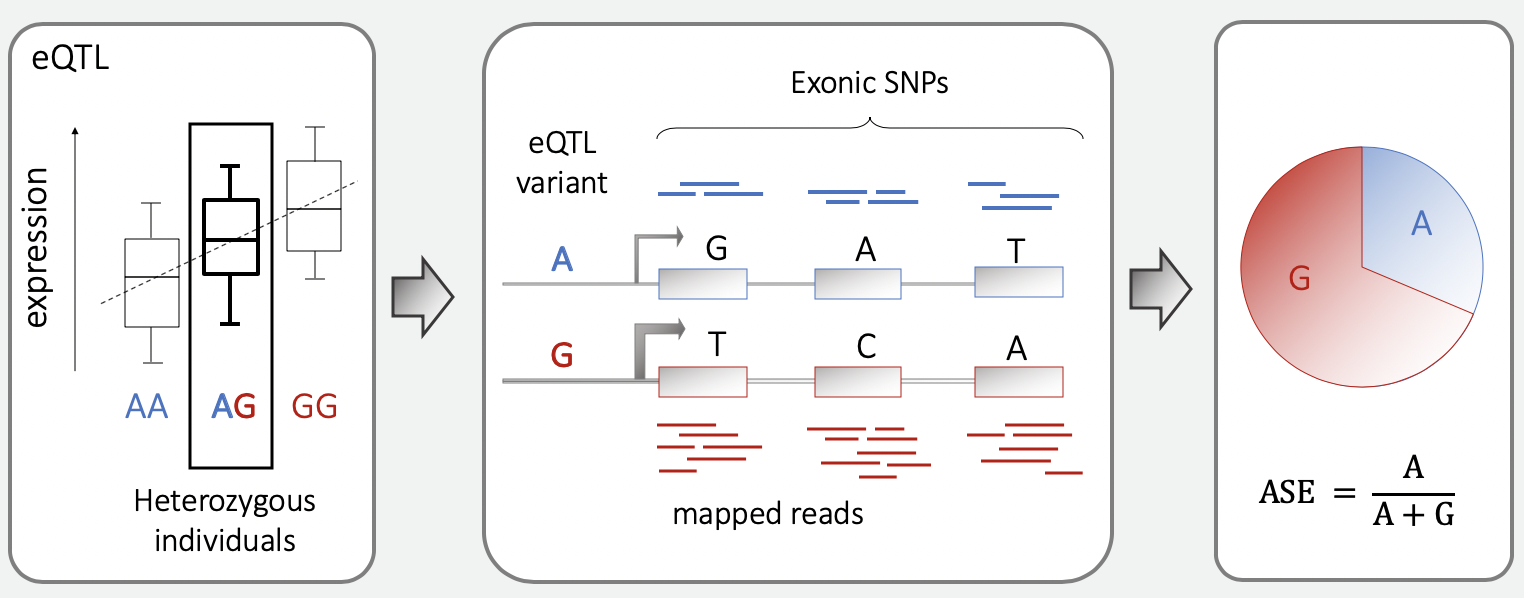
\includegraphics[width=15cm]{Chapter4/Fig/ASE.png}

% ASE quantifies the relative expression of one allele over the other. 
If one of these alleles is more responsive to a particular environmental factor (e.g. because of preferential transcription factor binding), then \gls{ase} is expected to vary consistently with that factor. 
This observation has previously been used to identify GxE interactions in gene expression across individuals \cite{knowles2017allele}. 
Critically, these \gls{ase} tests are internally matched, because potentially confounding batch effects and technical variation should affect both alleles in each cell similarly.
Additionally, this test increases power by reducing the number of parameters to estimate, i.e. instead of the standard test for interactions:  

\begin{equation*}
    \mathrm{expression} = \sum_{k=1}^{K} \mathbf{e}_k\alpha_k + \mathbf{g}\beta +
    \sum_{k=1}^{K} \mathbf{g} \odot \mathbf{e}_k\gamma_k + \boldsymbol{\psi},
\end{equation*}

where for each of K environments $\mathbf{e}_k$ two terms must be added (to account for E and GxE), resulting in (2*K + 2) parameters needing to be estimated (including one effect size $\beta$ and the variance explained by the noise term $\sigma_n^2$, from $\boldsymbol{\psi} \sim \mathcal{N}(\mathbf{0}, \sigma_n^2\mathbf{I_n})$), we can run:

\begin{equation*}
    \mathrm{ASE} = \sum_{k=1}^{K} \mathbf{e}_k\alpha_k + \boldsymbol{\psi}, 
\end{equation*}
where we can test directly the effect of the K environments on ASE and therefore only K+1 parameters need estimation (the K $\alpha_k$'s and $\sigma_n^2$).

\end{Comment}

% \newpage

% One obvious explanation for these subtle dynamic changes could be that they are simply reflecting changes in overall expression. \\

% \subsection{Sliding window}
% First, for visualisation purposes, 
% To visualise this,
% we used a sliding-window approach. 
% Because we need a rather large amount of cells to reliably estimate expression abundance for each individual, we slide a window containing 25\% of the cells along pseudotime by a step of 2.5\% cells.
% In each window, we considered average expression quantifications and estimate genetic effects using eQTL mapping, essentially performing the same analysis we performed in developmental stages in section \ref{sec:endodiff_eqtl}, now in each window.
% In parallel, we reassessed each eQTL in each window taking advantage of the full length transcript sequencing to measure \gls{ase}.
% Here, in each window, we quantified the deviation from 0.5 of the expression of the minor allele at the eQTL (ratio of reads phased to eQTL variants, Fig. \ref{fig:endodiff_sliding_window}). 
% Notably, ASE can be quantified in each cell and is independent of expression level, thus mitigating technical correlations between differentiation stage and genetic effect estimates (Box \ref{box:ase}). 

\begin{figure}[h]
\centering
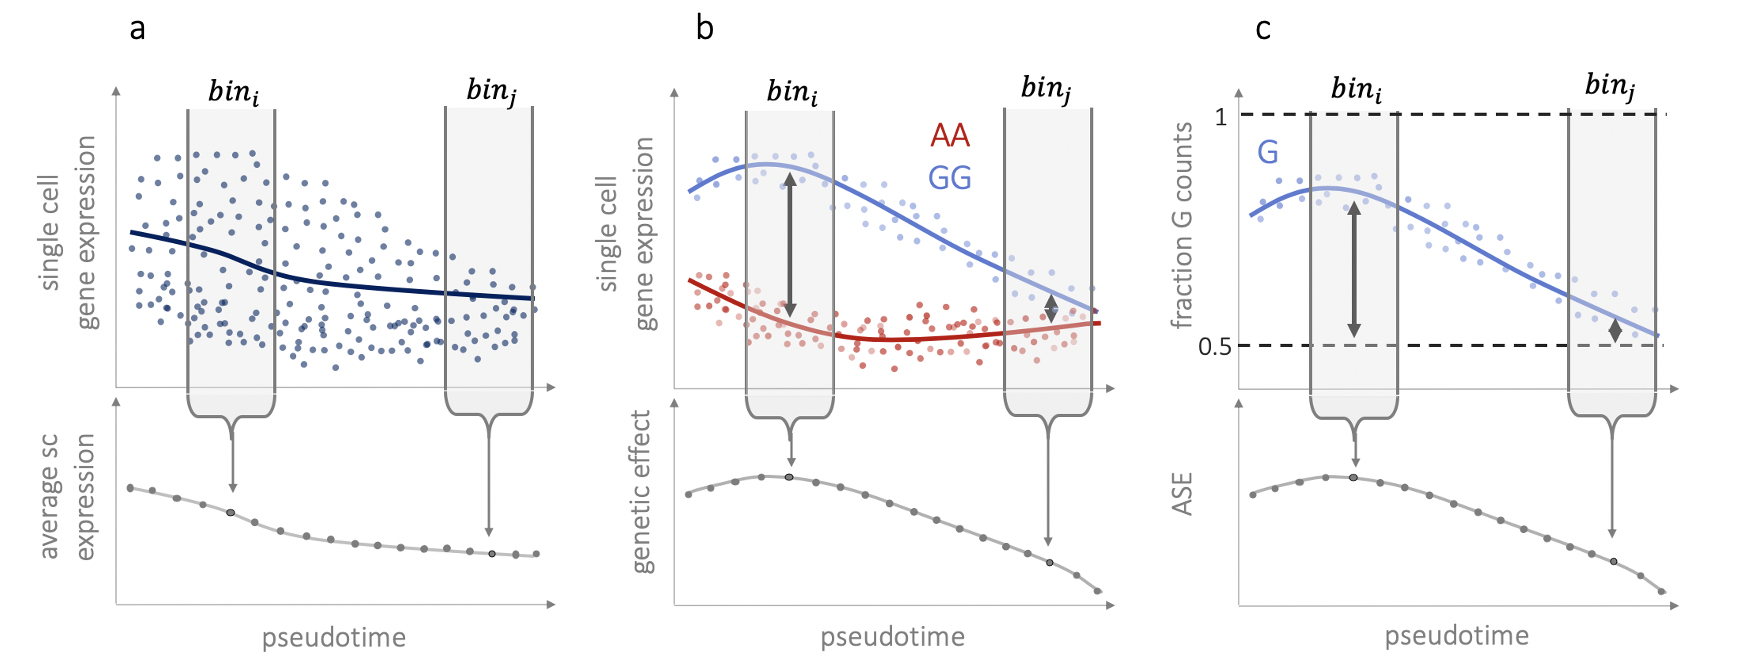
\includegraphics[width=15.5cm]{Chapter4/Fig/endodiff_running_average.png}
\caption[Schematic of the sliding window approach]{\textbf{Schematic of the sliding window approach.}\\
Cells are binned based on pseudotime ordering, to (a) quantify average expression, (b) perform eQTL mapping, and (c) quantify average ASE.
Each bin includes 25\% of cells, binned at incremental steps of 2.5\%.}
\label{fig:endodiff_sliding_window}
\end{figure}

Both methods result in a measure of genetic effect dynamics, i.e. changing strength of genetic effects along differentiation. 
Reassuringly, the two approaches were highly consistent across pseudotime (\textbf{Fig. \ref{fig:endodiff_dynamic_eqtl}}).
To explore this hypothesis, we clustered the top dynamic eQTL (FDR <1\%) jointly based on both the relative gene expression dynamics (global expression changes along pseudotime, quantified in sliding windows as above), and on the genetic effect dynamics (using ASE). 
This identified four basic dynamic patterns (\textbf{Fig. \ref{fig:endodiff_dynamic_eqtl}}): decreasing early (cluster A), decreasing late (cluster B), transiently increasing (cluster C), and increasing (cluster D). 
\begin{figure}[htbp]
\centering
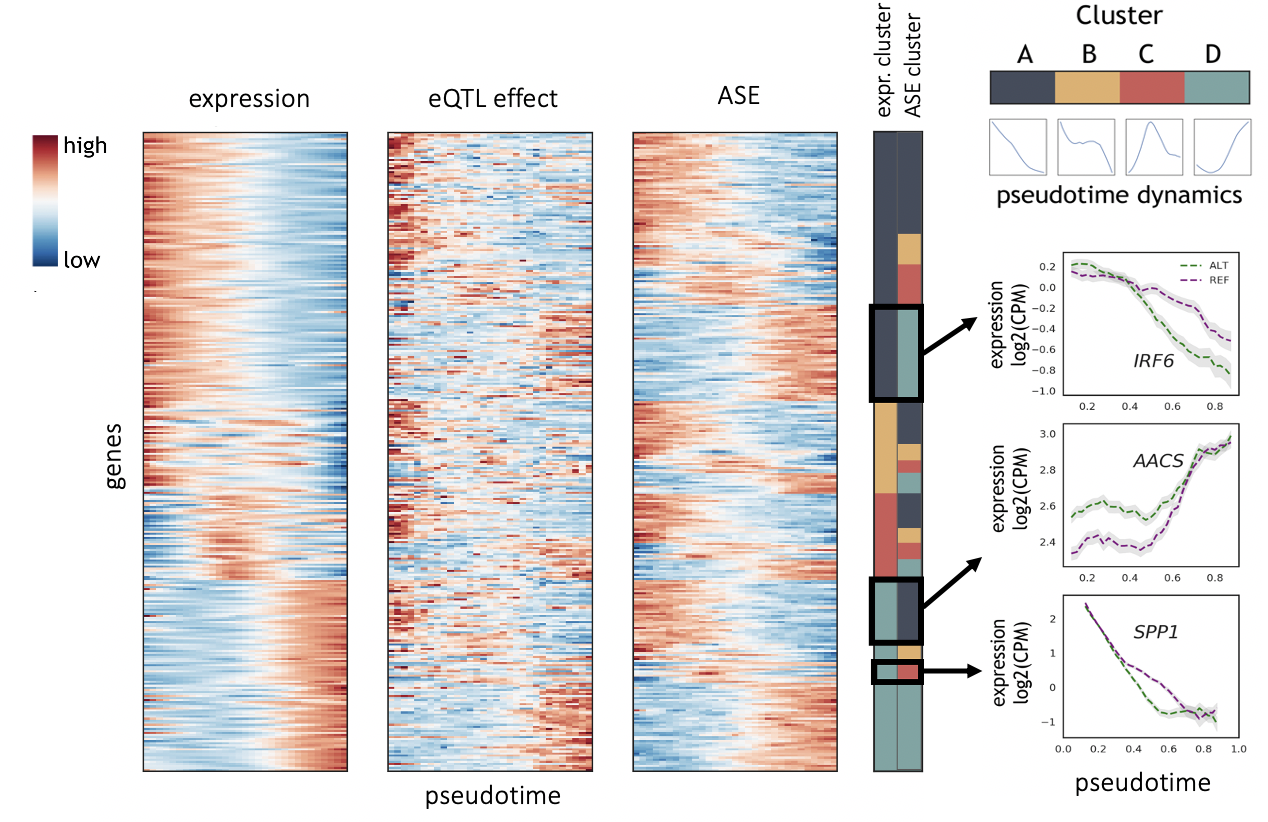
\includegraphics[width=15.5cm]{Chapter4/Fig/endodiff_pseudo_heatmap.png}
\caption[Dynamic eQTL]{\textbf{Dynamic eQTL.}\\
Clustered heatmap of global expression levels, eQTL effect sizes, and ASE across pseudotime for the top 311 genes with the strongest dynamic eQTL effects (FDR < 1\%; out of 785 at FDR < 10\%). 
For each gene, the dynamic profiles of gene expression and ASE were jointly grouped using clustering analysis, with 4 clusters. 
The membership of a genes's expression and ASE dynamics to one of these clusters is shown by colours in the right-hand panel. 
All values in the heatmaps are z-scores, normalised by gene (row). 
In particular, for ASE, average ASE values are plotted such that red indicates highest deviation from 0.5.
The diagram in the top right summarises the four identified cluster dynamics, displaying the average dynamic profile of each cluster, computed as the average across z-score normalised gene expression/ASE profiles. 
Selected examples of the dynamics of allele expression for different cluster-combinations are shown in the bottom right panel.
Shaded regions indicate standard error (+/- 1 SEM).
This figure is based on one by Daniel Seaton.}
\label{fig:endodiff_dynamic_eqtl}
\end{figure}
As expected, stage-specific eQTL were grouped together in particular clusters (e.g. defendo specific eQTL in cluster D, \textbf{Fig. \ref{fig:endodiff_dynamic_eqtl_enrichment}}). 
Notably, the dynamic profiles of gene expression and those of eQTL effects tended to be distinct, demonstrating that expression level is not the primary mechanism controlling variation in genetic effects. 
In particular, genetic effects were not most pronounced when gene expression was high (\textbf{Fig. \ref{fig:endodiff_dynamic_eqtl}}).
Distinct combinations of expression and eQTL dynamics result in different patterns of allelic expression over time. 
This is illustrated by the mesendoderm-specific eQTL for \textit{VAT1L}. 
Overall expression of \textit{VAT1L} decreases during differentiation, but expression of the alternative allele is repressed more quickly than that of the reference allele (\textbf{Fig. \ref{fig:endodiff_dynamic_eqtl}}). 
This illustrates how \textit{cis} regulatory sequence variation can modulates the timing of expression changes in response to differentiation, similar to observations previously made in \textit{C. elegans} using recombinant inbred lines \cite{francesconi2014effects}. 
In other cases, the genetic effect coincides with high or low expression, for example in the cases of \textit{THUMPD1} and \textit{PHC2} (\textbf{Fig. \ref{fig:endodiff_dynamic_eqtl}}). 
These examples illustrate how common genetic variation is closely linked to the dynamics of gene regulation. 
% \\

We next asked whether dynamic eQTL were located in specific regulatory regions. 
To do this, we evaluated the overlap of our identified dynamic eQTL with epigenetic marks defined using the hESC differentiation time series\footnote{using bulk, at equivalent time points along endoderm differentiation, see \textbf{section \ref{sec:endodiff_chipseq}} for methods.}(\textbf{Fig. \ref{fig:endodiff_dynamic_eqtl_enrichment}}). 
This revealed an enrichment of dynamic eQTL in enhancer (i.e. H3K27ac and H3K4me1), and promoter (H3K4me3) marks as compared to non-dynamic eQTL (i.e. eQTL we identified which did not display dynamic changes along pseudotime, \textbf{Fig. \ref{fig:endodiff_dynamic_eqtl_enrichment}}), consistent with these SNPs being located in active regulatory elements.

\vspace{2mm}

\begin{figure}[htbp]
\centering
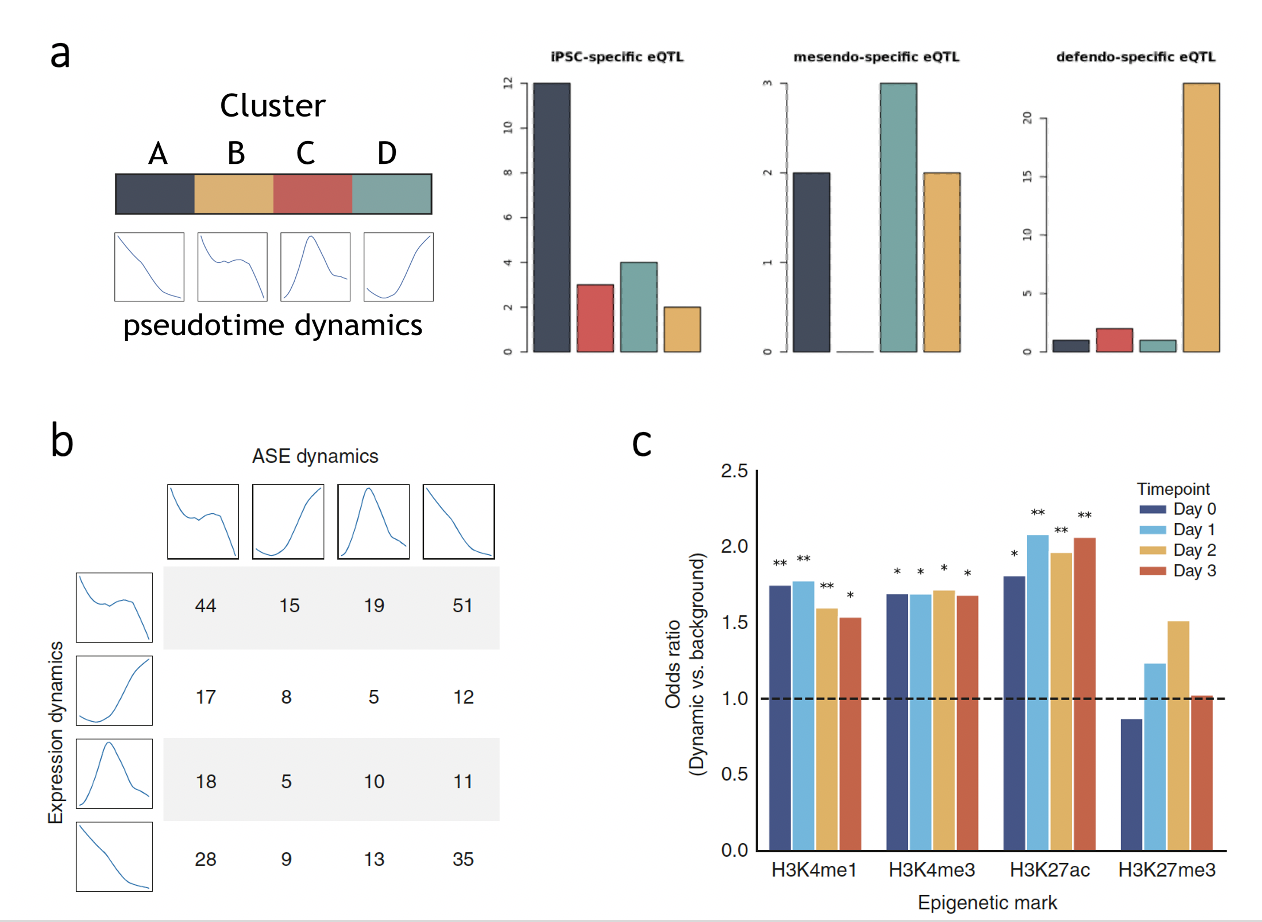
\includegraphics[width=15cm]{Chapter4/Fig/endodiff_dynamic_enrich.png}
\caption[Characterisation of dynamic eQTL]{\textbf{Characterisation of dynamic eQTL.}\\
(a) Summary of the identified cluster dynamics\footnotemark and assignment of stage-specific eQTLs to dynamic eQTL clusters. 
The numbers of each of the 3 classes of stage-specific eQTL (i.e. iPSC-, mesendo- , and defendo-specific eQTLs) that are assigned to each of the 4 dynamic eQTL clusters.
(b) Number of genes categorised by the combination of expression and ASE cluster from (a). 
Average dynamics of expression clusters (rows) and ASE clusters (columns) are shown.
(c) Overlap of dynamic eQTL variants from a with histone marks.
The odds ratio compared to the background of all other eQTL variants is shown (*p value < 0.01; **p value < $1x10^{-4}$; Fisher’s exact test).}
\label{fig:endodiff_dynamic_eqtl_enrichment}
\end{figure}

\footnotetext{displaying the average dynamic profile of each cluster, computed as the average values across z-score normalised gene expression/ASE profiles.}

\clearpage

\section{Cellular environment modulates eQTL effects}

Whilst differentiation was the main source of variation in the dataset, single cell RNA-seq profiles can be used to characterise cell-to-cell variation across a much wider range of cell state dimensions \cite{buettner2015computational, buettner2017f, fan2016characterizing}. 
Next, we identified sets of genes that varied in a co-regulated manner (co-expressed genes) using clustering.
In particular, grouping of genes by single-cell co-expression was performed using affinity propagation\footnote{The Pearson correlation across all cells was used as the similarity/‘affinity’ metric.} \cite{frey2007clustering}, as implemented by the Python scikit-learn library \cite{garreta2013learning}, using the top 8,000 highest expressed genes.
% (as judged by average expression across all cells)
This resulted in a set of 60 clusters of co-expressed genes. 
% \\
% The resulting modules were enriched for key biological processes such as cell differentiation, cell cycle state (G1/S and G2/M transitions), respiratory metabolism, and sterol biosynthesis (as defined by Gene Ontology annotations).
% GO enrichment of each cluster was performed by Fisher’s exact test in Python using
% GOATOOLS \cite{klopfenstein2018goatools}, and results are listed in Supplementary Data 6 (FDR 10\%).
Exemplar co-expression clusters were selected to represent 4 dimensions of
cellular state: cell cycle G1/S transition (cluster
10), cell cycle G2/M transition (cluster 30), cellular respiration (cluster 0), and
sterol biosynthesis (cluster 28). 
This selection was done according to two criteria: (i) strongest enrichment of relevant GO terms\footnote{GO enrichment of each cluster was performed by Fisher’s exact test in Python using GOATOOLS \cite{klopfenstein2018goatools}.}, and
% The co-expression clusters shown the largest over-representation of genes for the GO terms ‘G1/S transition of mitotic cell cycle’ (GO:0000082; cluster 10), ‘G2/M transition of mitotic cell cycle’ (GO:0000086; cluster 30), ‘respiratory electron transport chain’ (GO:0022904; cluster 0), and ‘sterol biosynthetic process’ (GO:0016126; cluster 28). 
(ii) a priori expectation of sources of cell-to-cell variation. 
Indeed, variation in cell cycle stage is a common feature of single-cell datasets \cite{buettner2015computational}, while variation in metabolic state during iPSC differentiation is well known \cite{xu2013mitochondrial}.
% The resulting modules were enriched for key biological processes such as cell differentiation, cell cycle state (G1/S and G2/M transitions), respiratory metabolism, and sterol biosynthesis (as defined by Gene Ontology annotations; Supplementary Data 6). 
These functional annotations were further supported by enrichment of relevant transcription factor binding (e.g. enrichment of \textit{SMAD3} and \textit{E2F7} targets in the differentiation and cell cycle modules, respectively). 
Additionally, expression of the cell differentiation module (cluster 6) was correlated with pseudotime, as expected (Pearson's R=0.62; \textbf{Fig. \ref{fig:endodiff_pseudotimes}}, panel d).\\

Using the same ASE-based interaction test as applied to identify dynamic eQTL, reflecting ASE variation across pseudotime, we assessed how the genetic regulation of gene expression responded to these cellular contexts. 
Briefly, we tested for genotype by environment (GxE) interactions using a subset of four co-expression modules as markers of cellular state, while accounting for effects that can be explained by interactions with pseudotime:

% Here, we applied similar concepts to single cell RNA-seq, testing for the influence of cellular environmental factors (i.e., cellular processes) on ASE in individual cells. 

\begin{equation}\label{eq:endodiff_ase_gxe}
    \mathrm{ASE} = \alpha_1 \mathrm{pseudotime} + \alpha_2 \mathrm{pseudotime}^2 + \beta\mathrm{factor} + \boldsymbol{\psi},
\end{equation}

where the test performed is: $H_1: \beta \neq 0$ (using a likelihood ratio test), and $\mathrm{factor}$ represented one of the four co-expression modules, 
% (two of which quantify cell cycle state: G1/S and G2/M transitions, and two metabolic pathway activity: respiratory metabolism and sterol biosynthesis), 
and was quantified as the normalised mean expression levels in each cell across all genes in the cluster.
% were taken as quantitative measures of cell cycle state (G1/S and G2/M transitions) and metabolic pathway activity (respiratory metabolism and sterol biosynthesis). 
This approach extends previous work using ASE to discover GxE interactions \cite{knowles2017allele, moyerbrailean2016high}, taking advantage of the resolution provided by single-cell data. \\

\begin{figure}[h]
\centering
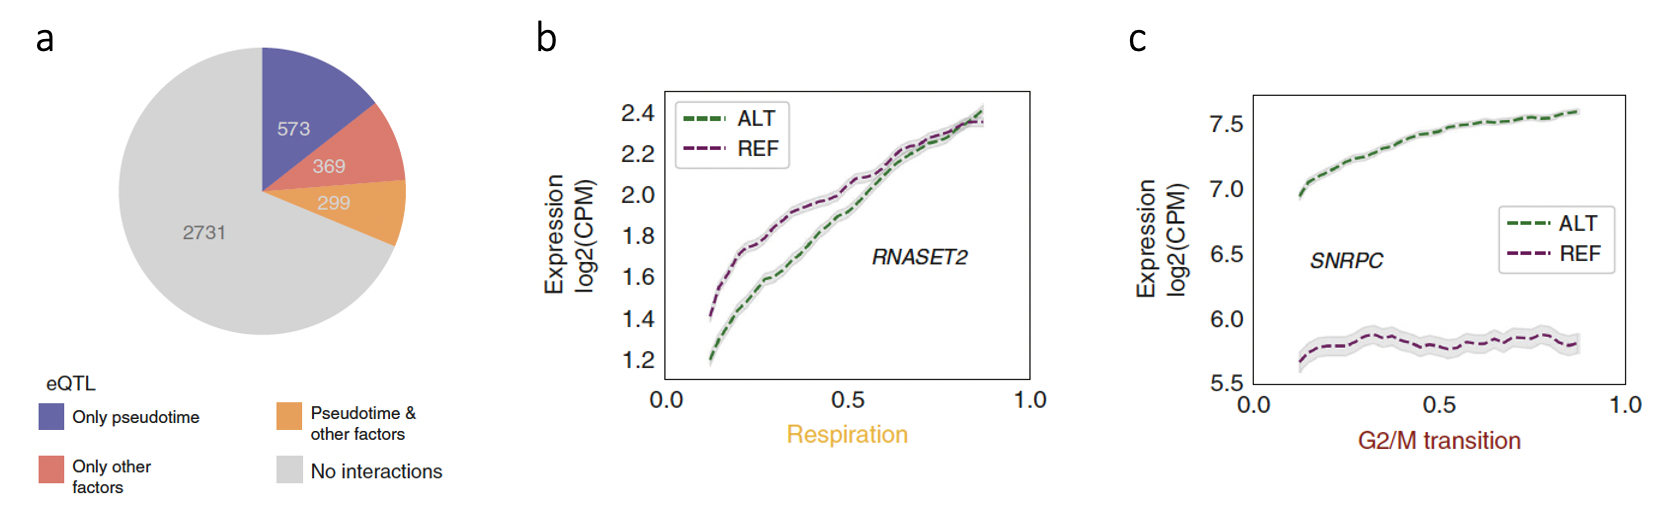
\includegraphics[width=15.5cm]{Chapter4/Fig/endodiff_GxE.png}
\caption[Allele-specific expression reveals interactions with fundamental cellular processes]{\textbf{Allele-specific expression reveals interactions with fundamental cellular processes.}\\
(a) Results summary: numbers of eQTL identified as displaying GxE interactions with pseudotime (purple), displaying GxE interactions with other cellular contexts but not with pseudotime, (after appropriately accounting for pseudotime, red), displaying GxE interactions with both pseudotime and at least one other cellular context (yellow), and displaying no GxE interactions at all (grey). 
Significance is assessed at FDR < 10\%.
(b) ASE variation for two example eQTL SNPs that show GxE interactions (FDR < 10\%) and tag cancer-associated GWAS variants. 
The eQTL for \textit{RNASET2} (rs2247315) tags a risk variant for basal cell carcinoma, and its effect size is modulated by cellular respiration, while the eQTL for \textit{SNRPC} (rs9380455) tags a risk variant for prostate cancer and is responsive to the G2/M transition of the cell cycle. 
For each cell, cellular contexts were inferred using GO annotations of co-expression modules. 
Shaded regions indicate standard error (+/- 1 SEM).}
\label{fig:endodiff_gxe}
\end{figure}

We identified 668 eQTL that had an interaction effect with at least one factor (at FDR < 10\%), with many of these eQTL having no evidence for an interaction with differentiation.
Indeed, 369 genes had no association with pseudotime, but responded to at least one other factor. 
Conversely, of the 872 dynamic eQTL, 299 were also associated with GxE effects with other factors, whereas 573 were exclusively associated with pseudotime.\\

These interactions encompass regulatory effects on genes and SNPs with important functional roles. Specifically, 95 interaction eQTL variants overlap with variants previously identified in genome-wide association studies (GWAS, LD $r^2>0.8$). 
For example, the effect size of a \textit{RNASET2} eQTL is sensitive to cellular respiratory metabolic state. 
This eQTL SNP is in LD ($r^2=0.86$) with a GWAS risk variant for basal cell carcinoma \cite{chahal2016genome}. Furthermore, an eQTL for \textit{SNRPC} showed sensitivity to the G2/M state, and is in LD ($r^2=0.92$) with a GWAS risk variant for prostate cancer \cite{schumacher2018association} (\textbf{Fig. \ref{fig:endodiff_gxe}}). 
These cellular factors vary not only across cells in the experiments considered here, but also across cells \textit{in vivo}, across individuals, and across environments. 
Thus, these examples illustrate the versatility of our single cell dataset and how it can provide regulatory information about variants in contexts beyond early human development.\\

Finally, we explored whether we could detect higher order interaction effects, where the genetic effect varies with a cellular state in different ways along differentiation, effectively testing for genotype x environment x environment (GxExE) interactions. 
To this end, we fitted a linear model with fixed effects for differentiation and each of the factors, plus a combined term (factor x pseudotime):

\begin{equation}\label{eq:endodiff_ase_gxexe}
    \mathrm{ASE} = \alpha_1 \mathrm{pseudotime} + \alpha_2 \mathrm{pseudotime}^2 + \alpha_3\mathrm{factor} + \beta (\mathrm{pseudotime}*\mathrm{factor}) + \boldsymbol{\psi},
\end{equation}

where we test: $H_1: \beta \neq 0$. \\

This approach identified 176 genes with significant higher order (GxExE) interactions between a genetic variant, pseudotime, and at least one other factor. 
For example, an eQTL for \textit{EIF5A}, was responsive to G2/M state, especially early in differentiation, as measured using ASE (\textbf{Fig. \ref{fig:endodiff_gxexe}}). 
% These results highlight the context-specificity of eQTL, and the power of \gls{scrnaseq} in dissecting this specificity within one set of experiments.

\begin{figure}[h]
\centering
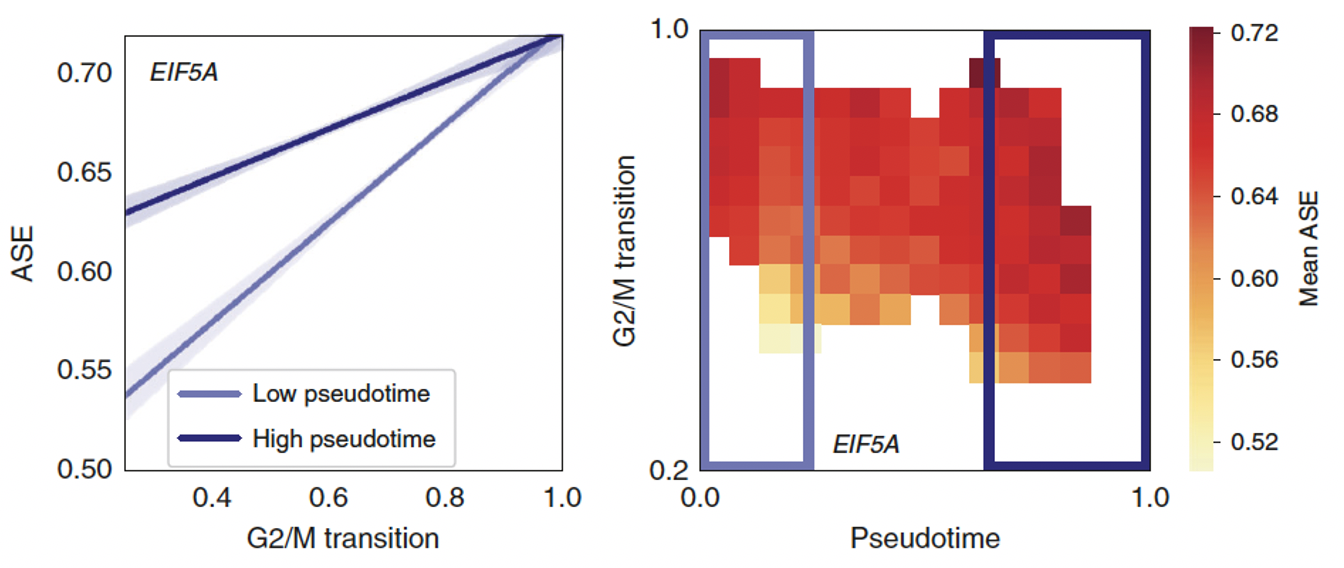
\includegraphics[width=15.5cm]{Chapter4/Fig/endodiff_GxExE.png}
\caption[Second order GxE interactions with fundamental cellular processes]{\textbf{Second order GxE interactions with fundamental cellular processes.}\\
Figure by Daniel Seaton.
Higher order interaction example: an eQTL variant for \textit{EIF5A} (rs7503161) is affected by a GxExE higher order interaction with both pseudotime and the G2/M transition. 
Left panel: effects of G2/M transition on ASE for cells with low and high pseudotime. 
Regression lines are indicated with 95\% confidence intervals for the 30\% of cells with lowest and highest pseudotime values. 
Right panel: heatmap of averaged ASE for cells falling within the specified windows of pseudotime and G2/M transition. 
Only values for windows containing more than 30 cells are shown (n=6,423 cells in total).}
\label{fig:endodiff_gxexe}
\end{figure}

\newpage

\section{Early markers are predictive of differentiation efficiency}
\label{sec:endodiff_differentiation_efficiency}

The final piece of analysis we performed on this dataset was based on the observation that iPSC lines have been shown to vary in their capacity to differentiate, as demonstrated by previous studies \cite{bock2011reference}.
This motivated us to look at whether we could detect clear differences in the ability to differentiate among our 126 lines.
We used the average pseudotime value at the latest time point considered (day3) as a measure of differentiation efficiency in our analysis.
This was motivated by the observation that there was significant variation across cell lines, which remained consistent across replicate differentiation experiments of the same cell line (\textbf{Fig. \ref{fig:endodiff_differentiation_efficiency}}, n=33).
Exploiting the scale of our study and the pooled experimental design, we set out to look for potential markers of differentiation efficiency that are accessible prior to differentiation.

\begin{figure}[h]
\centering
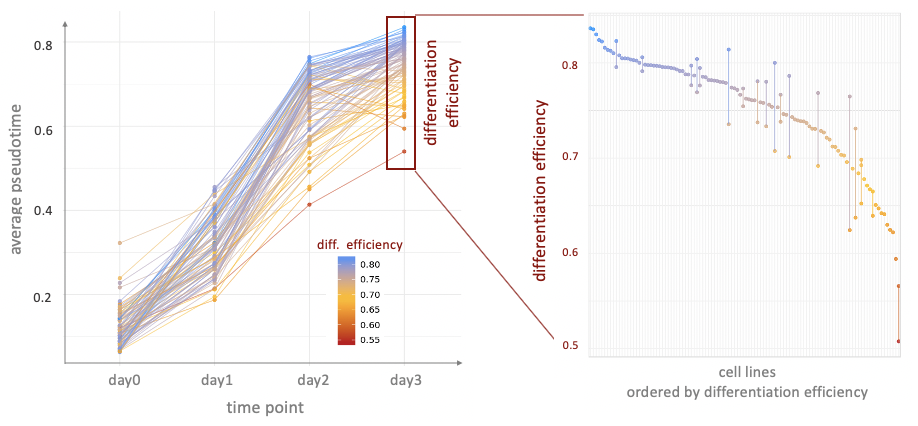
\includegraphics[width=15.5cm]{Chapter4/Fig/endodiff_differentiation_efficiency.png}
\caption[Line-to-line variation in differentiation efficiency]{\textbf{Line-to-line variation in differentiation efficiency.}\\
Variation in differentiation efficiency across cell lines. 
Left: average pseudotime values for each line, showing trajectories over time for 98 cell lines, coloured by differentiation efficiency. 
Shown are 98 cell lines (out of 126) for which we had sufficient data at all time points (> 10 cells at each time point). 
Differentiation efficiency of a cell line was defined as its average pseudotime value across all cells on day 3.
Right: differentiation efficiency across cell lines (points), and consistency of individual cell lines differentiated in multiple experiments (vertical bars, n=33).}
\label{fig:endodiff_differentiation_efficiency}
\end{figure}

First, we looked for genetic markers.
% If we had access to data for several hundreds or better thousands individuals, we could perform a \gls{gwas} with differentiation efficiency as the trait of interest and consider all variants genome-wide.
Given our small sample size and consequent low statistical power, we limited our pool to the set of 4,422 eQTL lead variants at any of the three developmental stages\footnote{rather than testing all variants genome-wide. 
Note that this would be essentially a \gls{gwas}, and normally a \gls{gwas} is considered to be well powered at around 1,000 individuals.}.
We tested each variant for association with differentiation efficiency using a linear mixed model, similar to eq. \eqref{eq:Linear_mixed_model}:

\begin{equation}\label{eq:LMM_differentiation_efficiency_prediction}
    \mathrm{Differentiation} \ \mathrm{efficiency} = \beta*\mathrm{Marker} + \mathrm{Experiment} + \mathrm{Donor} + \boldsymbol{\psi},
\end{equation}

where $\mathrm{Experiment}$ is a random effect grouping sets of samples from the same experiment, and $\mathrm{Donor}$ is a random effect grouping samples from the same donor (and cell line). 
Here, a $\mathrm{Marker}$ is a genetic variant (i.e., eQTL SNP), and it is modelled as a fixed effect, with corresponding weight $\beta$.
The models were fitted using the lme4 package in R \cite{bates2014fitting}, and significance was determined using a likelihood ratio test ($H_1: \beta \neq 0$).
This identified only one significant association, with the eQTL variant for \textit{DPH3}, at FDR < 10\%.
In an attempt to validate this finding, we performed an additional set of differentiations in HipSci iPSC lines derived from individuals that were not part of the variant discovery, selected based on genotype at this variant (n=20). 
In these experiments, differentiation efficiency was measured by the percentage of CXCR4+ cells on day3:

\begin{equation}
    \mathrm{\% CXCR4+} = \beta*\mathrm{Marker} + \boldsymbol{\psi}.
\end{equation}

While the direction of effect was consistent, the association was not statistically significant (p value = 0.24, Student’s t-test), probably reflecting low power at this sample size. 
We conclude that larger sample sizes will be required to conclusively identify genetic predictors of \textit{in vitro} differentiation efficiency.\\

Secondly, we asked whether levels of gene expression at the iPSC stage (prior to differentiation) could represent molecular markers of differentiation efficiency.
We used the same model as in eq. \eqref{eq:LMM_differentiation_efficiency_prediction}, with $\mathrm{Marker}$ in this case indicating the expression of genes at iPSC stage.
This revealed 38 associations at FDR < 10\%, out of 11,231 genes tested (\textbf{Fig. \ref{fig:endodiff_manhattan_differentiation}}).


\begin{figure}[h]
\centering
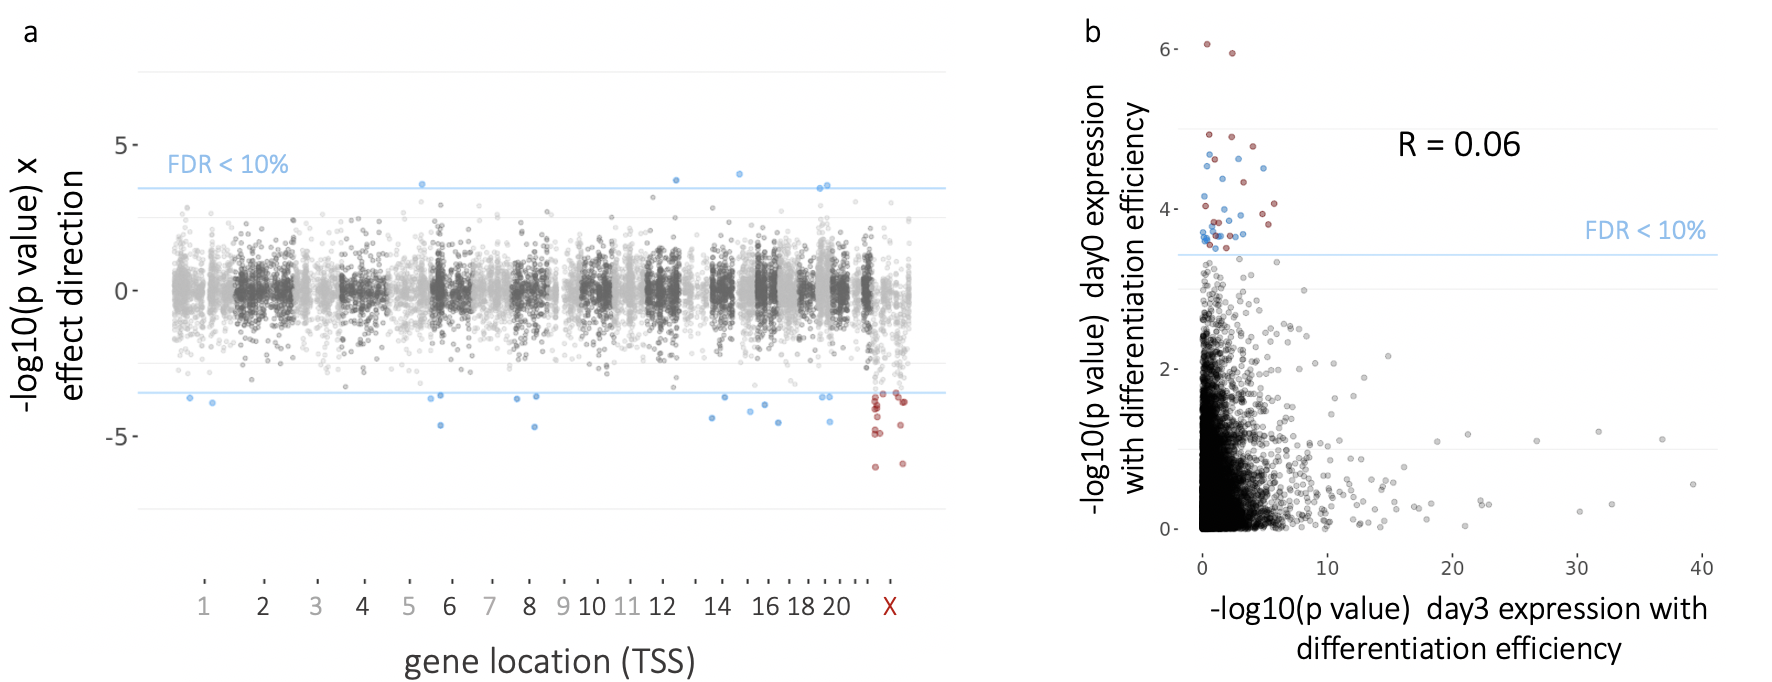
\includegraphics[width=15.5cm]{Chapter4/Fig/endodiff_diff_eff_manhattan.png}
\caption[Associations between iPSC gene expression levels and differentiation efficiency]{\textbf{Associations between iPSC gene expression levels and differentiation efficiency.}\\
(a) Genome-wide analysis to identify markers of differentiation efficiency (defined as average pseudotime at day3), considering iPSC gene expression levels. 
Displayed are negative log (nominal) p values signed by the direction of the effect. 
The horizontal blue lines denote the significance threshold (FDR = 10\%, Benjamini-Hochberg adjusted). 
Significant associations are shown in blue for autosomal genes and in red for X chromosome genes. 
(b) Scatter plot comparing, for all genes, the statistical significance of associations with differentiation efficiency for their expression on day0 and day3. 
The y axis shows the association between the expression of the gene on day0 (i.e. in iPSC) and differentiation efficiency of cell lines. 
The x axis shows the association between the expression of the gene on day3 and differentiation efficiency. 
The correlation between these associations is R = 0.06, demonstrating that the genes identified as predictive markers of differentiation efficiency (i.e. those with high values on the y axis) are not the genes that define differentiation capacity (i.e. those with high values on the x axis). 
Significance measured as -log10(p value). 
Significant genes are coloured as in (a): autosomal genes in blue, X chromosome genes in red.}
\label{fig:endodiff_manhattan_differentiation}
\end{figure}

A subset of those genes (9/38) were also observed when using independent bulk RNA-seq data from the same cell lines to look for an association between gene expression and differentiation efficiency (nominal p value < 0.05). 
We note that expression of these marker genes is largely orthogonal to pseudotime itself, i.e. these are not genes that vary across pseudotime, and only as a consequence of that are associated with differentiation efficiency (which is defined as average pseudotime at day3, \textbf{Fig. \ref{fig:endodiff_manhattan_differentiation}}). 
We noted that 17 of the 38 differentiation-associated genes were located on the X chromosome, reflecting a significant enrichment of X chromosome genes (24.5-fold enrichment, p value = $8x10^{-16}$, Fisher’s exact test). 
For all of the X chromosome genes, higher expression was associated with reduced differentiation efficiency (\textbf{Fig. \ref{fig:endodiff_manhattan_differentiation}}). 
The majority of these associations (14/17) persisted when performing the same analysis for only female lines (p value < 0.05), indicating variation beyond differences between sexes. 
\\
% To formally evaluate whether donor sex had a significant effect on differentiation, we fitted the following linear mixed model:

% \begin{equation}
%     \mathrm{Differentiation} \ \mathrm{efficiency} = \beta*\mathrm{Sex} + \mathrm{Experiment} + \mathrm{Donor} + \boldsymbol{\psi},
% \end{equation}

% where $\mathrm{Sex}$ is modelled as a fixed effect and tested for significance using likelihood ratio test ($H_1: \beta \neq 0$), and $\mathrm{Experiment}$ and $\mathrm{Donor}$ were modelled as random effects, as above.
These results are consistent with observations made by other groups, showing that X chromosome reactivation is a marker of poor differentiation capacity for iPSCs in general (see \textbf{page \pageref{sec:ipsc_somatic_cell}}) \cite{anguera2012molecular, patel2017human}. 
We did not identify any other striking patterns in the genes identified other than the reported over-representation of chromosome X genes, partly due to a small sample size.

% mention the other failed experiment?
% \newpage

\section{Discussion}

% make more personal
% add other work

% single cell eQTL there has been Monique's paper (refer to previous chapter) but this is larger scale \cite{van2018single} and in new cell types (vs blood)
% remind briefly of sc vs bulk eQTL (which should be in discussion from Chapter 
% \ref{chapter3}
% 3)
% dynamic eQTL \cite{francesconi2014effects,strober2019dynamic} but not sc and few individuals (and not humans, respectively)
% GxE using ASE \cite{knowles2017allele} but here at sc resolution
% previous work on differentiation efficiency briefly and hint at next chapter

Here, we generated a map of early endoderm differentiation across human \gls{ipsc} lines from 125 unrelated individuals  (\textbf{Fig. \ref{fig:endodiff_experimental_design}, \ref{fig:endodiff_pca}}).
This offers a unique and powerful tool which allows the interrogation of the role of genetic heterogeneity in early human development. \\

First, we characterise the effects of common genetic variants on gene expression at three distinct developmental stages, adapting methods traditionally used for bulk RNA-sequencing to single cell expression data (\textbf{Fig \ref{fig:endodiff_stage_eqtl}} and see \textbf{Chapter \ref{chapter3}} for ample discussion on single cell eQTL mapping).
This was one of the first single cell eQTL mapping studies (after \cite{wills2013single} and \cite{van2018single}), and the first with over 100 individuals (previous largest sample size was 45).
Additionally, we mapped eQTL in mesendoderm and definitive endoderm cells, providing the first eQTL maps (single cell or otherwise) at these key developmental stages. 
In this application, the benefit of using single cell expression profiles resides mainly in the ability to define homogeneous cell populations in an unbiased manner, resulting in a higher number of detected eQTL (\textbf{Fig. \ref{fig:endodiff_stage_eqtl}}).
We can also use this tool to start assessing the amount of sharing of \gls{eqtl} signal between closely related developmental stages.
In particular, we found that about one third of the identified \glspl{eqtl} at any given stage was specific to that stage (\textbf{Fig. \ref{fig:endodiff_stage_specific_eqtl}}).\\

\textcolor{blue}{While relevant from a developmental biology perspective, the discretisation into three developmental stages (iPSC, mesendoderm, definitive endoderm) is somewhat arbitrary, as the differentiation trajectory clearly appears as a continuum (\textbf{Fig. \ref{fig:endodiff_pca}, \ref{fig:endodiff_stages}}).
To reflect this,} we exploited this resource to identify hundreds of dynamic eQTL, i.e. eQTL whose strength is modulated by differentiation time in a continuous manner (\textbf{Fig. \ref{fig:endodiff_dynamic_eqtl}}).
Reassuringly, we found that eQTL dynamics were largely independent of total gene expression dynamics (\textbf{Fig. \ref{fig:endodiff_dynamic_eqtl_enrichment}}).
These findings nicely complement results from a similar study \cite{strober2019dynamic}, where they identify eQTL in cells from iPSC lines that are differentiated toward cardiomyocytes across more time points (16) but for fewer individuals (19).
\textcolor{blue}{I note that we cannot completely rule out that differentiation itself may be genetically regulated, although the results presented in \textbf{section \ref{sec:endodiff_differentiation_efficiency}}, where we found no common genetic variant associated with differentiation efficiency indicates that those effects, if present, are probably negligible for our dynamic eQTL analysis. }\\

Additionally, we extend the concept of context-specific eQTL \cite{fairfax2012genetics, fairfax2014innate, knowles2017allele} to single cell resolution, identifying eQTL which are modulated by specific cellular states including cell cycle phases and preferential metabolic pathways, thus fully utilising the power of single-cell transcriptomics.
% (for more discussion on this point see \textbf{Chapter 
% \ref{chapter6}}).
% 6).
These results highlight the power of using a single cell approach for eQTL mapping, which allows detailed annotation of changing eQTL effects across heterogeneous cell types and cell states, with the ability to better interpret the context-specific role of individual genetic variants (\textbf{Figures \ref{fig:endodiff_gxe}, \ref{fig:endodiff_gxexe}}). \\

A further advantage of the application of single-cell transcriptomics in this study was to enable the pooling strategy. 
While the feasibility of pooling samples has already been demonstrated for PBMCs \cite{kang2018multiplexed}, in this study we have extended this to cell lines differentiated together in culture. 
This strategy provided higher throughput, and enabled the characterisation of line-to-line variability in terms of differentiation efficiency in a controlled setting. 
While the differentiation protocol considered here (to definitive endoderm) is short and efficient, other protocols (e.g. to generate neurons \cite{tao2016neural}) are much more challenging, making a pooling strategy useful for scaling up these protocols to population-scale (this aspect is further discussed in the next chapter, \textbf{Chapter \ref{chapter5}}).
\textcolor{blue}{There are some possible drawbacks of a pooled design. 
For example, paracrine signalling \cite{muller2016distinguishing} could affect differentiation dynamics of cell lines grown together and obscure genetic effects.} Additionally, although we have considered replicates of the same line across different experimental pools, our study is based on a single \gls{ipsc} line per donor. 
In the future, experimental designs may consider multiple lines per donor, which, however, would require a different barcoding scheme as these cannot be discriminated
using genetic barcodes. 
As a result of this experimental design, we cannot definitively distinguish between donor and cell line effects.\\

In summary, our results demonstrate the power of combining \gls{ipsc} line pooling and \gls{scrnaseq} to investigate development and genetics \textit{in vitro}. 
Sorting of cells along different cellular states allows eQTL  context-specificity to be probed in detail across many axes of cellular variation. 
The \gls{scrnaseq} readouts also provide a rich description of the progress of differentiation over time across different cell lines. \\

This work acts as a proof of principle study, where we establish the feasibility of combining a pooled experimental design, differentiation of human iPSCs and \gls{scrnaseq} readouts across several individuals.
In the next chapter (\textbf{Chapter 
\ref{chapter5}}),
% 5), 
we apply a similar set up to a larger scale and much more complex differentiation protocol, with cells differentiating to dopaminergic neurons, which are preferentially lost in Parkinson's disease.
This other protocol generates more mature cell types, which are directly disease-relevant, and thus allows us to characterise the genetic component of differentiation across a larger spectrum of human development and disease.
Additionally, we will have more power to explore differences in differentiation capacity across more lines and after a much longer differentiation period.

